%%%%%%%%%%%%%%%%%%%%%%%%%%%%%%%%%%%%%%%%%%%%%%%%%%%%%%%%%%%%%%%%%%%%%%%%
% Plantilla TFG/TFM
% Escuela Politécnica Superior de la Universidad de Alicante
% Realizado por: Jose Manuel Requena Plens
% Contacto: info@jmrplens.com / Telegram:@jmrplens
%%%%%%%%%%%%%%%%%%%%%%%%%%%%%%%%%%%%%%%%%%%%%%%%%%%%%%%%%%%%%%%%%%%%%%%%

\chapter{Experimentos}
\label{experimentos}

\FloatBarrier
\section{Diseño experimental}

En esta sección se presentan los experimentos realizados para evaluar la capacidad predictiva de los modelos aplicados al crecimiento trimestral del PIB (variación QoQ\%) de España, Francia e Italia.

Los experimentos de XGBoost (Bloques 0--2) utilizan como fuente única el dataset \texttt{dataset\_\allowbreak{}panel\_\allowbreak{}v1.parquet}, que integra los indicadores macroeconómicos descargados de la API de Eurostat para los tres países. Esta decisión garantiza la consistencia metodológica entre bloques y elimina posibles discrepancias derivadas del uso de datasets distintos. Los modelos de referencia lineales, limitados a España, se evalúan sobre el mismo periodo de prueba. Con el fin de evitar fuga de información, únicamente se emplean variables rezagadas como predictores en todos los casos.

Se define una partición temporal coherente con un escenario real de predicción:

\begin{itemize}
    \item Conjunto de entrenamiento: 2009Q2 -- 2023Q3
    \item Conjunto de prueba: 2023Q4 -- 2025Q3 (8 trimestres)
\end{itemize}

La evaluación se realiza fuera de muestra, utilizando como métricas el error absoluto medio (MAE) y la raíz del error cuadrático medio (RMSE). Ambas permiten cuantificar el error en puntos porcentuales de crecimiento trimestral.

Cabe señalar que el conjunto de prueba comprende únicamente 8 trimestres por país. Este tamaño reducido implica que las métricas obtenidas pueden verse afectadas de forma significativa por uno o dos errores puntuales, y que las diferencias entre modelos deben interpretarse con cautela: lo que aquí se observa apunta a tendencias y patrones, pero no permite extraer conclusiones estadísticamente robustas sobre la superioridad de un modelo frente a otro.

Los experimentos se estructuran en dos niveles. Primero se evalúan dos modelos de regresión lineal sobre España como punto de referencia interpretable. A continuación se presentan tres bloques de experimentos con XGBoost: el Bloque~0 entrena modelos independientes por país; el Bloque~1 combina los datos de los tres países en un único modelo de panel; el Bloque~2 extiende el Bloque~1 incorporando la variable de país como feature explícita mediante codificación \textit{one-hot}.

En cada bloque de XGBoost se comparan dos configuraciones de features:

\begin{itemize}
    \item \textbf{Modelo base}: utiliza únicamente desempleo e inflación rezagados (\texttt{unemployment\_\allowbreak{}rate\_\allowbreak{}l1}, \texttt{inflation\_\allowbreak{}qoq\_\allowbreak{}pct\_\allowbreak{}l1}).
    \item \textbf{Modelo ampliado}: incorpora además los dos retardos del propio PIB, el índice de producción industrial y el índice de comercio minorista (\texttt{gdp\_\allowbreak{}qoq\_\allowbreak{}pct\_\allowbreak{}l1}, \texttt{gdp\_\allowbreak{}qoq\_\allowbreak{}pct\_\allowbreak{}l2}, \texttt{ipi\_\allowbreak{}qoq\_\allowbreak{}pct\_\allowbreak{}l1}, \texttt{retail\_\allowbreak{}qoq\_\allowbreak{}pct\_\allowbreak{}l1}).
\end{itemize}

% ══════════════════════════════════════════════════════════════════════
\FloatBarrier
\section{Modelos de referencia --- Regresión lineal}

Antes de introducir los modelos de \textit{gradient boosting}, se evalúan dos modelos de
regresión lineal ordinaria (OLS) sobre España. Su propósito es doble: por un lado,
establecer un punto de referencia interpretable contra el que medir la ganancia de los
modelos más complejos; por otro, comprobar si una relación lineal simple entre los
indicadores macroeconómicos rezagados y el crecimiento del PIB es suficiente para capturar
la dinámica del ciclo económico en el periodo de prueba.

A diferencia de los bloques experimentales, estos modelos se limitan a España y utilizan
la misma partición temporal que el resto de experimentos
(entrenamiento: 2009Q2--2023Q3; prueba: 2023Q4--2025Q3).

\subsection{Modelo univariante}

El modelo más simple posible para este problema consiste en predecir el crecimiento del
PIB a partir únicamente de la tasa de desempleo retardada un trimestre:

\[
\widehat{\text{gdp\_qoq\_pct}}_t = \beta_0 + \beta_1 \cdot \text{unemployment\_rate}_{t-1}
\]

Los resultados sobre el conjunto de prueba son MAE = 0.428 p.p. y RMSE = 0.465 p.p.

Como se aprecia en la Figura~\ref{fig:lin_es_pred}, el modelo produce predicciones
prácticamente constantes a lo largo del horizonte de prueba, con valores que oscilan
alrededor de 0.35 p.p. independientemente del trimestre. Esto se debe a que la tasa de
desempleo española en el periodo de prueba varía dentro de un rango estrecho (10.5--12.1\%),
lo que se traduce en una señal predictiva casi invariante. El modelo, en la práctica,
predice un crecimiento próximo a la media de entrenamiento en todos los trimestres.

El gráfico de errores (Figura~\ref{fig:lin_es_err}) confirma esta limitación: todos los
errores son positivos, lo que indica que el modelo subestima sistemáticamente el
crecimiento real durante el periodo de prueba. Esto apunta a que la
relación lineal entre desempleo y PIB no logra capturar la dinámica de recuperación y estabilización
que caracteriza el ciclo económico español en el periodo analizado.

\begin{figure}[H]
\centering
\begin{minipage}[t]{0.48\textwidth}
    \centering
    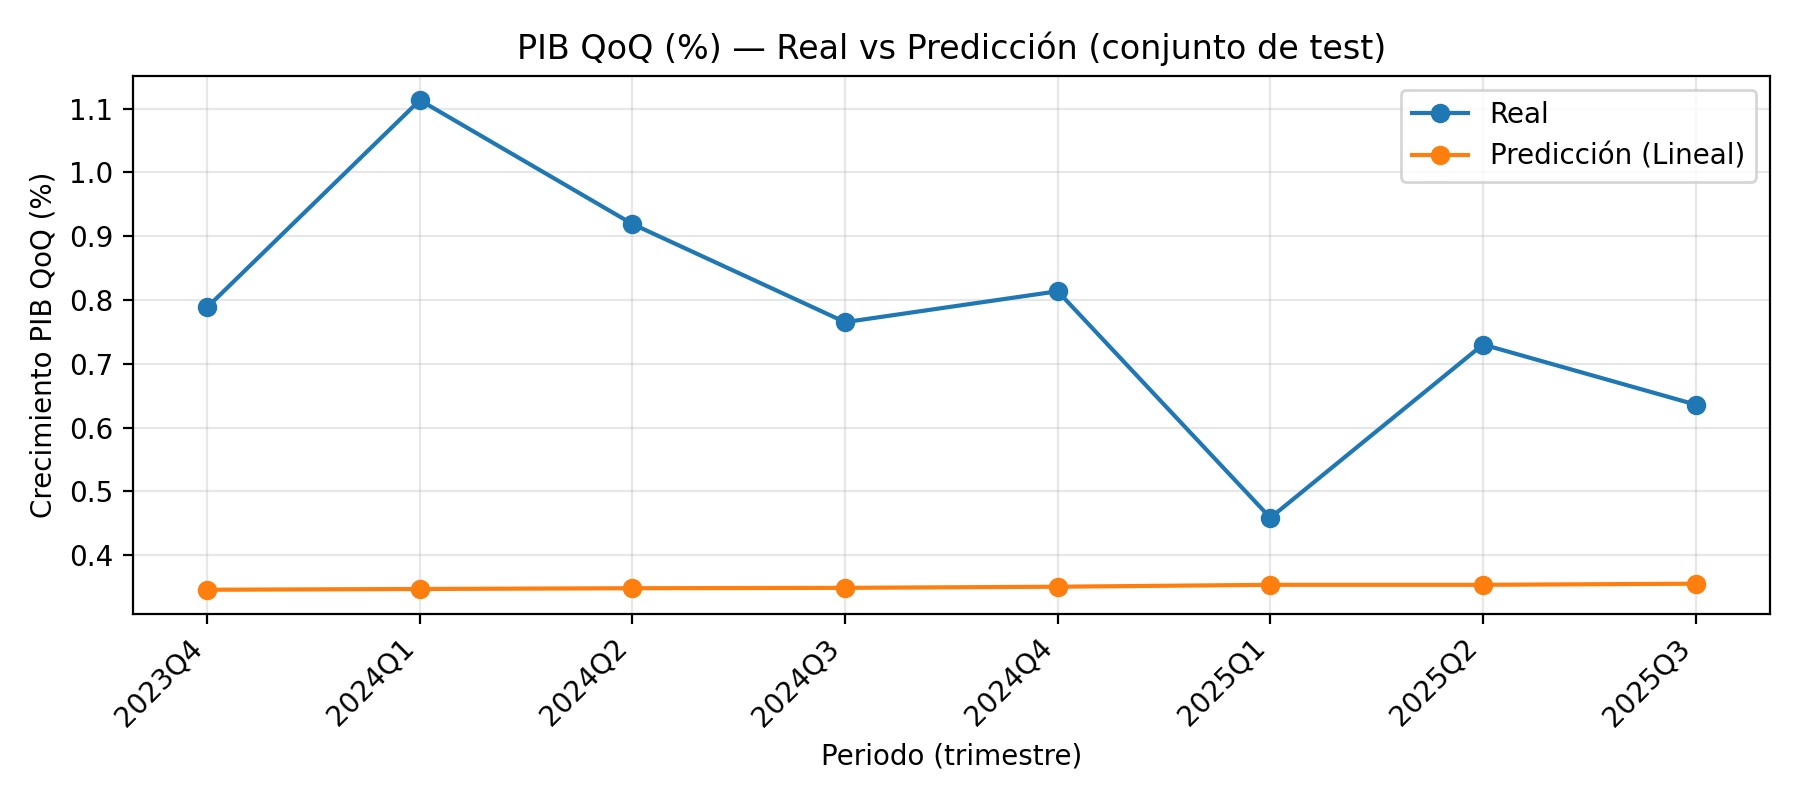
\includegraphics[width=\textwidth]{figures/linear_es_real_vs_pred.png}
    \caption{PIB QoQ real vs predicción -- Lineal univariante (ES, test)}
    \label{fig:lin_es_pred}
\end{minipage}\hfill
\begin{minipage}[t]{0.48\textwidth}
    \centering
    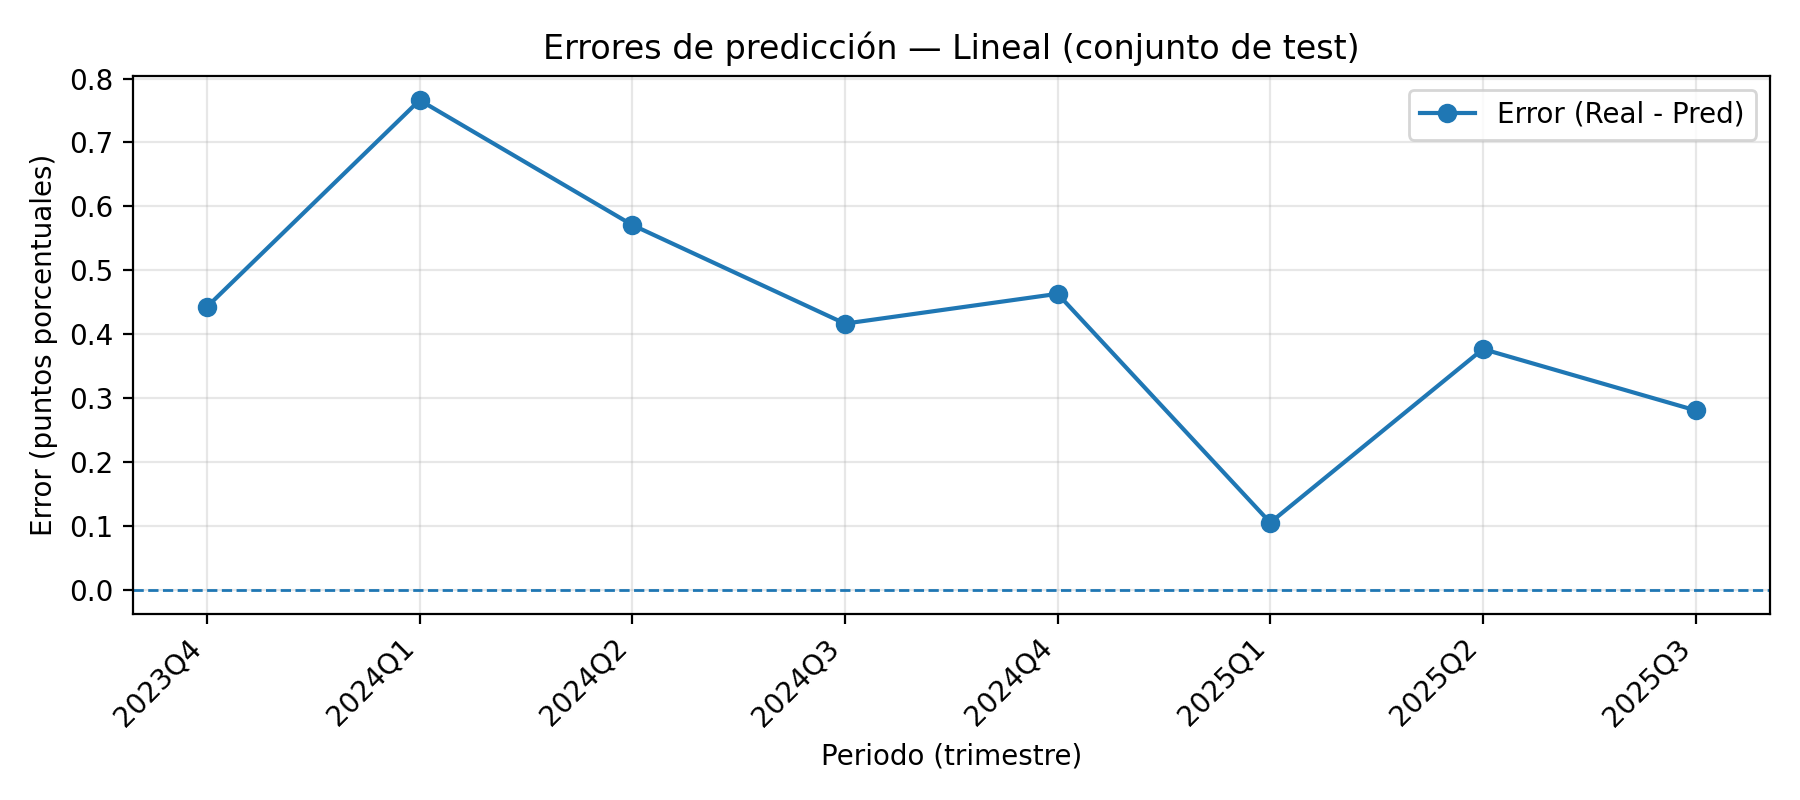
\includegraphics[width=\textwidth]{figures/linear_es_errors.png}
    \caption{Errores de predicción -- Lineal univariante (ES, test)}
    \label{fig:lin_es_err}
\end{minipage}
\end{figure}

\subsection{Modelo multivariante}

El segundo modelo añade la inflación trimestral rezagada como segunda variable predictora:

\[
\widehat{\text{gdp\_qoq\_pct}}_t = \beta_0 + \beta_1 \cdot \text{unemployment\_rate}_{t-1}
+ \beta_2 \cdot \text{inflation\_qoq\_pct}_{t-1}
\]

Contra lo que cabría esperar, los resultados empeoran: MAE = 0.476 p.p. y RMSE = 0.578 p.p.,
frente a los 0.428 y 0.465 del modelo univariante.

La causa reside en la naturaleza de la relación entre inflación y PIB: no es lineal ni
estable en el tiempo. Durante periodos de baja inflación, el crecimiento y la inflación
pueden moverse en la misma dirección; durante periodos de choque de precios como 2022--2023,
la relación se invierte. Un modelo OLS estima un único coeficiente $\beta_2$ promediando
estas fases opuestas, lo que introduce ruido en lugar de señal. La Figura~\ref{fig:lin_multivar_pred}
muestra que la incorporación de la inflación provoca mayor volatilidad en las predicciones
---visible en los errores de la Figura~\ref{fig:lin_multivar_err}---, con un error puntual
de 0.92 p.p. en 2024Q4, trimestre en que la inflación rezagada tomó un valor negativo
inusual que el modelo interpretó erróneamente como señal contractiva.

\begin{figure}[H]
\centering
\begin{minipage}[t]{0.48\textwidth}
    \centering
    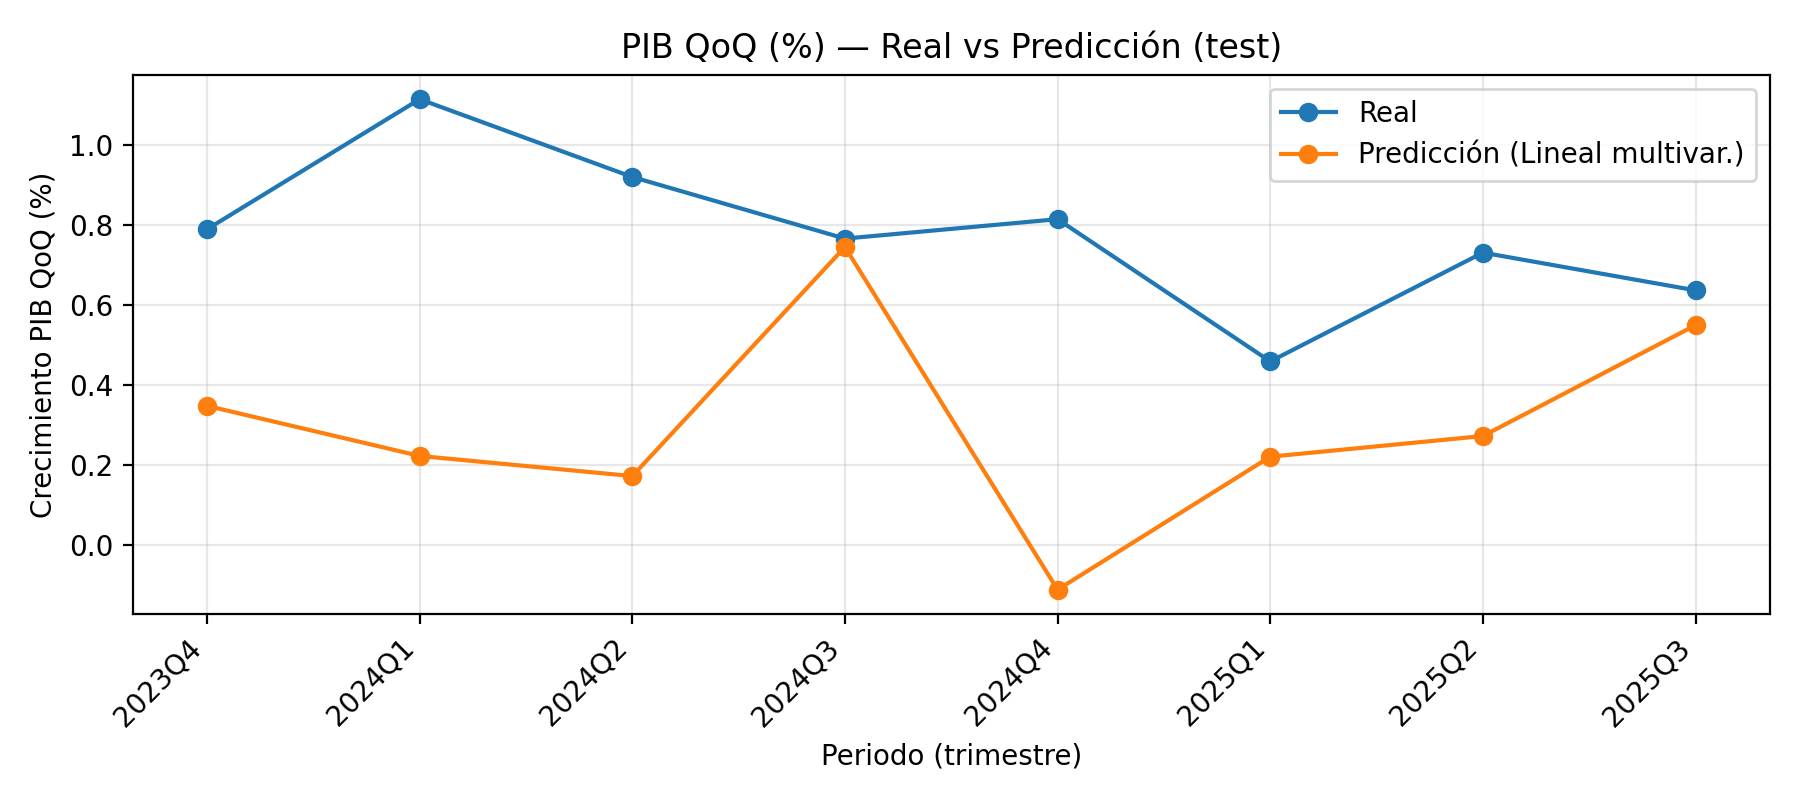
\includegraphics[width=\textwidth]{figures/linear_multivar_es_real_vs_pred.png}
    \caption{PIB QoQ real vs predicción -- Lineal multivariante (ES, test)}
    \label{fig:lin_multivar_pred}
\end{minipage}\hfill
\begin{minipage}[t]{0.48\textwidth}
    \centering
    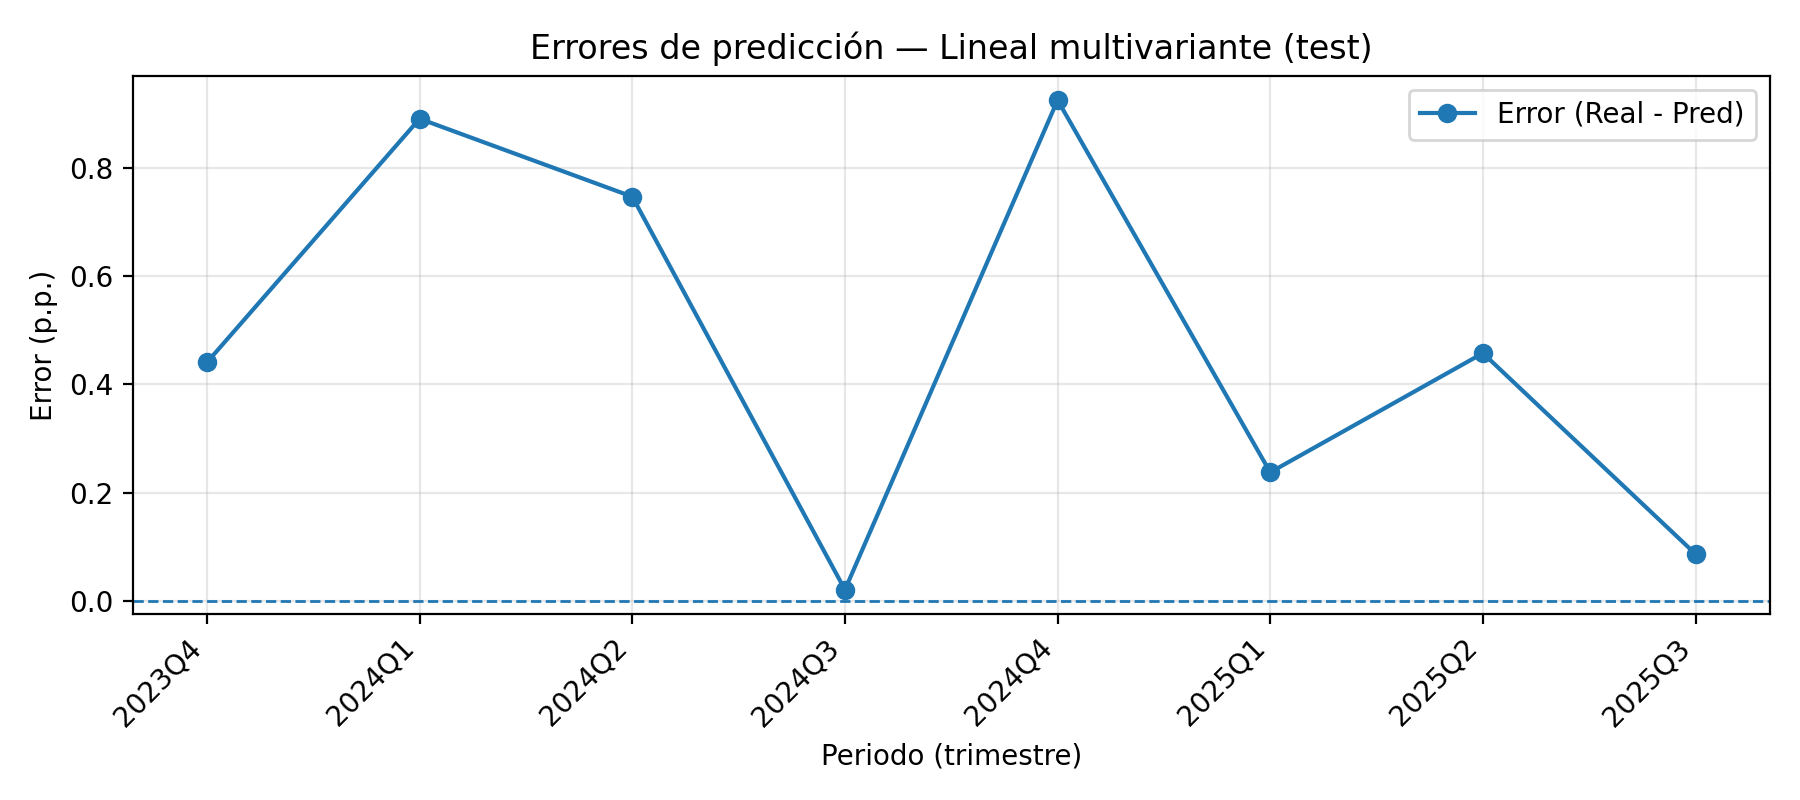
\includegraphics[width=\textwidth]{figures/linear_multivar_es_errors.png}
    \caption{Errores de predicción -- Lineal multivariante (ES, test)}
    \label{fig:lin_multivar_err}
\end{minipage}
\end{figure}

\subsection{Síntesis y comparación con el modelo de referencia}

\begin{table}[H]
\centering
\caption{Resultados de los modelos de regresión lineal -- España}
\label{tab:linear}
\small
\begin{tabular}{lccc}
\hline
\textbf{Modelo} & \textbf{Features} & \textbf{MAE} & \textbf{RMSE} \\
\hline
Lineal univariante   & 1 & 0.428 & 0.465 \\
Lineal multivariante & 2 & 0.476 & 0.578 \\
\hline
\end{tabular}
\end{table}

El análisis revela dos limitaciones estructurales de la regresión lineal para este problema.
Primera: con pocas variables y una relación débil o inestable con el PIB, el modelo tiende
a predecir un valor casi constante próximo a la media de entrenamiento, incapaz de capturar
la variabilidad trimestral real. Segunda: añadir variables no mejora necesariamente el
resultado si la relación con el objetivo no es lineal y estable en el tiempo; en ese caso,
el coeficiente estimado promedia fases de signo opuesto y degrada la predicción.

Estos resultados motivan el uso de XGBoost, que puede capturar relaciones no lineales entre
las variables y el PIB, adaptar su respuesta según el nivel de las variables (lo que OLS
no puede hacer con un único coeficiente), y aprovechar combinaciones de indicadores sin
imponer una forma funcional rígida. Los experimentos de los Bloques 0--2 apuntan a que
este salto en complejidad se traduce en una mejora del error de predicción en la mayor parte de los escenarios analizados.

% ══════════════════════════════════════════════════════════════════════
\FloatBarrier
\section{Bloque 0 --- Modelos por país}

\textbf{Idea principal:} entrenar modelos independientes por país permite establecer una línea de referencia, y los resultados sugieren que no existe una configuración universalmente mejor: la configuración óptima parece depender de la economía analizada, lo que apunta a diferencias estructurales en la predictibilidad del ciclo de cada país.

El primer bloque de experimentos entrena y evalúa los modelos de forma independiente para cada país, utilizando únicamente los datos propios de cada economía. Este enfoque permite establecer los resultados de referencia para cada país antes de explorar estrategias que combinen información de múltiples economías.

Los resultados obtenidos en el conjunto de prueba para los tres países son los siguientes:

\begin{table}[H]
\centering
\caption{Comparativa de modelos XGBoost por país -- Bloque 0}
\label{tab:bloque0}
\small
\begin{tabular}{lcccccc}
\hline
 & \multicolumn{2}{c}{\textbf{España}} & \multicolumn{2}{c}{\textbf{Francia}} & \multicolumn{2}{c}{\textbf{Italia}} \\
\textbf{Modelo} & \textbf{MAE} & \textbf{RMSE} & \textbf{MAE} & \textbf{RMSE} & \textbf{MAE} & \textbf{RMSE} \\
\hline
XGBoost base     & 0.314 & 0.365 & 0.441 & 0.486 & 0.761 & 0.813 \\
XGBoost ampliado & 0.796 & 1.285 & 0.193 & 0.208 & 0.344 & 0.455 \\
\hline
\end{tabular}
\end{table}

\FloatBarrier
\subsection{España}

El modelo base obtiene el mejor resultado para España (MAE 0.314), superando claramente al modelo ampliado (MAE 0.796). Como se observa en la Figura~\ref{fig:xgb_base_es}, el modelo base reproduce razonablemente la tendencia del crecimiento trimestral, manteniéndose en el rango positivo y siguiendo de forma aproximada la evolución real.

En cambio, la Figura~\ref{fig:xgb_ext_es} muestra que el modelo ampliado produce una predicción anómala de $-2.5$ puntos porcentuales en 2023Q4, cuando el valor real fue de $0.8$ p.p. Este error en el primer trimestre del conjunto de prueba es el principal responsable del alto RMSE del modelo ampliado, y apunta a un problema de sobreajuste sobre los retardos del PIB durante el entrenamiento.

\begin{figure}[H]
\centering
\begin{minipage}[t]{0.48\textwidth}
    \centering
    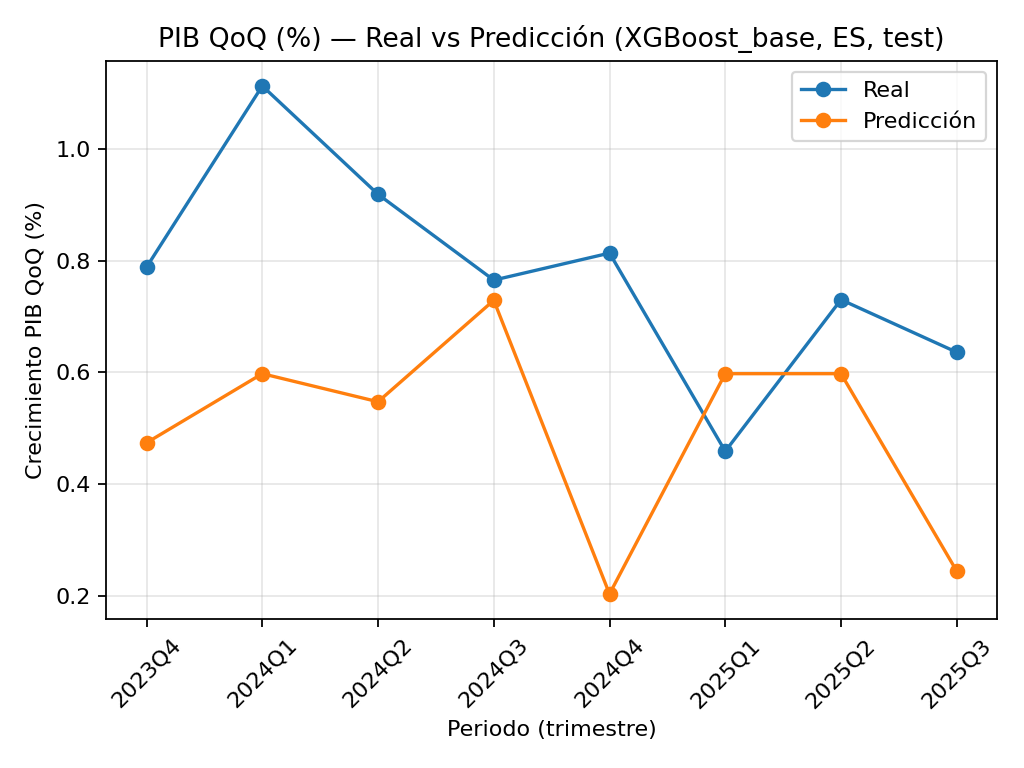
\includegraphics[width=\textwidth]{figures/bloque 0/xgboost_base_es_real_vs_pred.png}
    \caption{PIB QoQ real vs predicción -- XGBoost base (ES, test)}
    \label{fig:xgb_base_es}
\end{minipage}\hfill
\begin{minipage}[t]{0.48\textwidth}
    \centering
    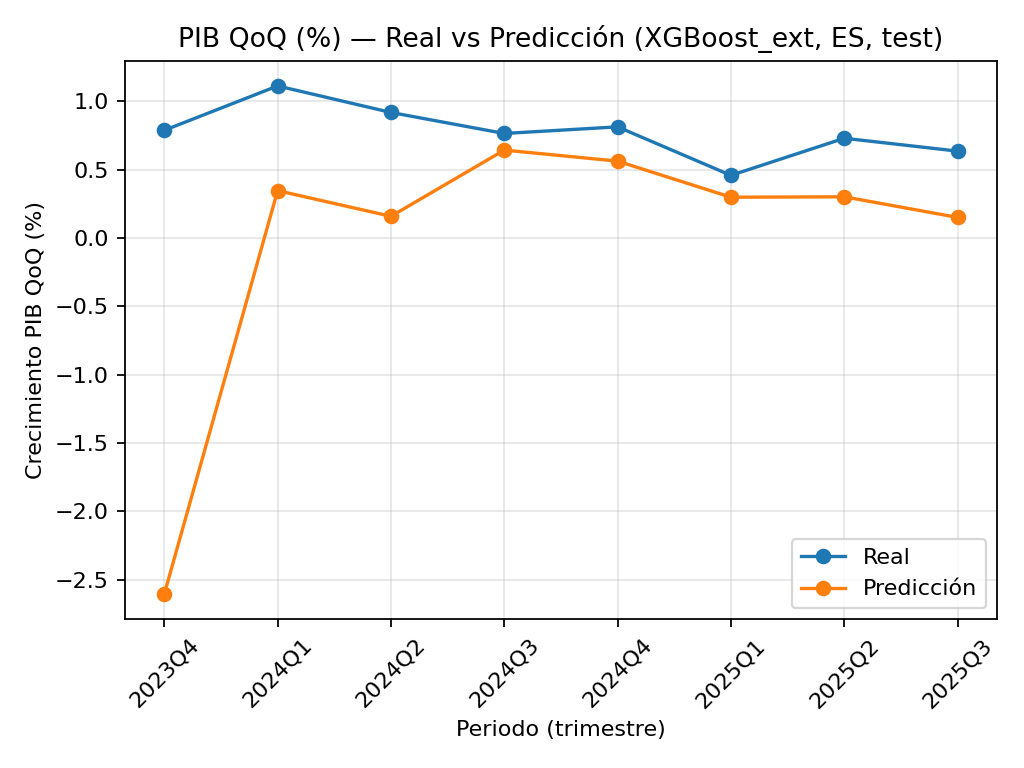
\includegraphics[width=\textwidth]{figures/bloque 0/xgboost_ext_es_real_vs_pred.png}
    \caption{PIB QoQ real vs predicción -- XGBoost ampliado (ES, test)}
    \label{fig:xgb_ext_es}
\end{minipage}
\end{figure}

\FloatBarrier
\subsection{Francia}

Francia presenta el patrón opuesto: el modelo ampliado (MAE 0.193) supera con claridad al modelo base (MAE 0.441). La Figura~\ref{fig:xgb_base_fr} muestra que el modelo base oscila de forma pronunciada alrededor de los valores reales sin capturar bien la tendencia. El modelo ampliado, visible en la Figura~\ref{fig:xgb_ext_fr}, sigue de forma más suave la evolución real, aunque tiende a sobreestimar ligeramente el crecimiento en los trimestres centrales del periodo de prueba.

\begin{figure}[H]
\centering
\begin{minipage}[t]{0.48\textwidth}
    \centering
    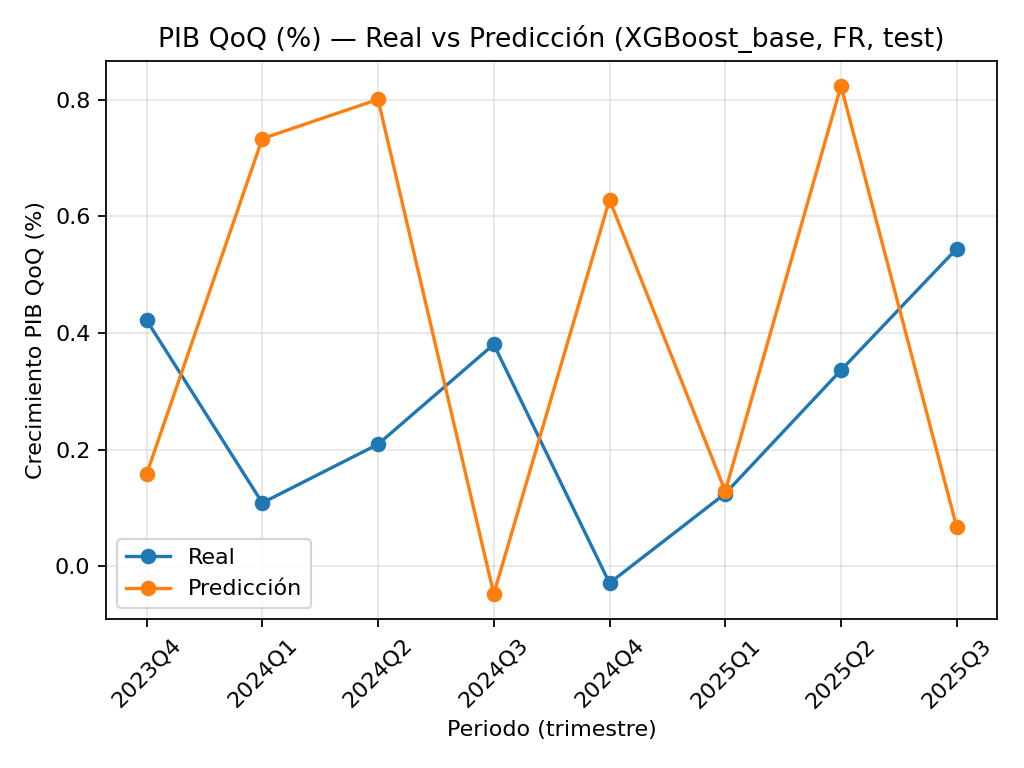
\includegraphics[width=\textwidth]{figures/bloque 0/xgboost_base_fr_real_vs_pred.png}
    \caption{PIB QoQ real vs predicción -- XGBoost base (FR, test)}
    \label{fig:xgb_base_fr}
\end{minipage}\hfill
\begin{minipage}[t]{0.48\textwidth}
    \centering
    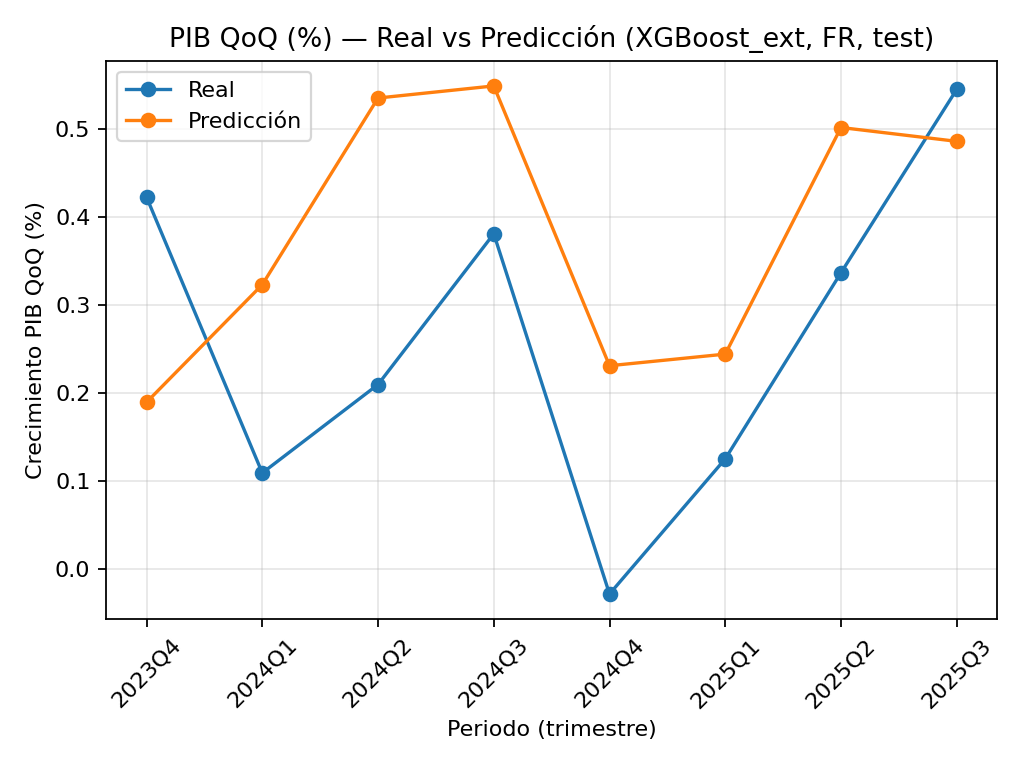
\includegraphics[width=\textwidth]{figures/bloque 0/xgboost_ext_fr_real_vs_pred.png}
    \caption{PIB QoQ real vs predicción -- XGBoost ampliado (FR, test)}
    \label{fig:xgb_ext_fr}
\end{minipage}
\end{figure}

\FloatBarrier
\subsection{Italia}

Italia es el país con mayor error en el modelo base (MAE 0.761), con predicciones que se alejan notablemente de los valores reales en varios trimestres, como se aprecia en la Figura~\ref{fig:xgb_base_it}. El modelo ampliado mejora considerablemente (MAE 0.344), aunque la Figura~\ref{fig:xgb_ext_it} muestra una predicción anómala de $-0.85$ p.p. en 2024Q2 cuando el valor real fue de $0.2$ p.p., patrón similar al observado en España con el modelo ampliado.

\begin{figure}[H]
\centering
\begin{minipage}[t]{0.48\textwidth}
    \centering
    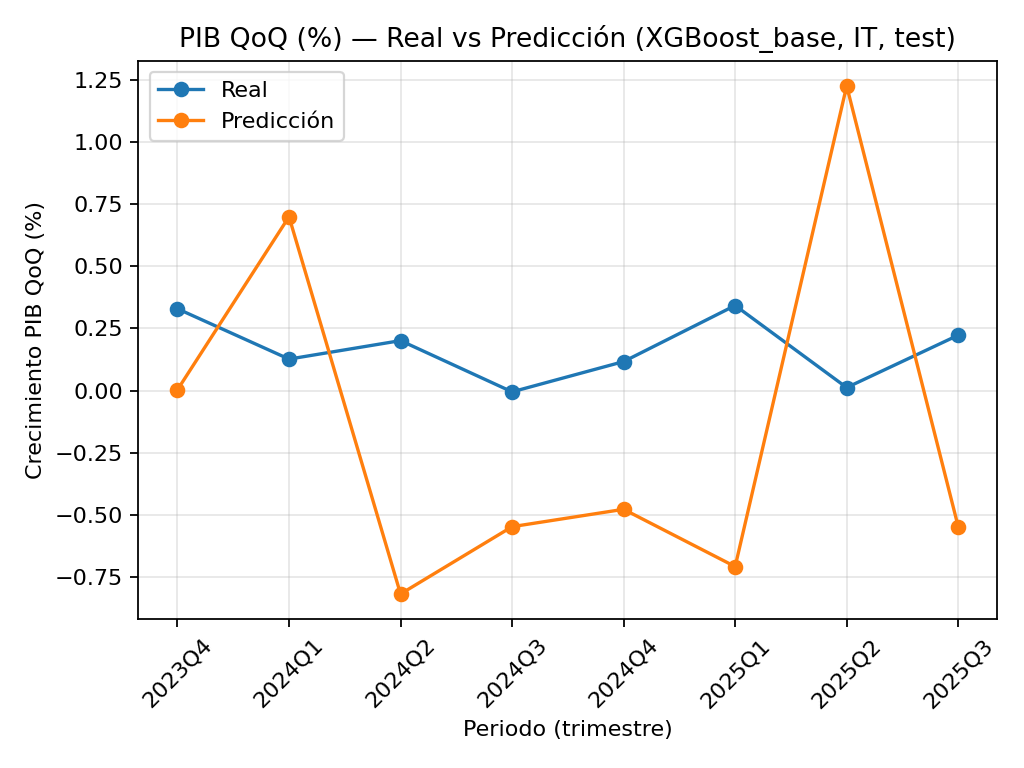
\includegraphics[width=\textwidth]{figures/bloque 0/xgboost_base_it_real_vs_pred.png}
    \caption{PIB QoQ real vs predicción -- XGBoost base (IT, test)}
    \label{fig:xgb_base_it}
\end{minipage}\hfill
\begin{minipage}[t]{0.48\textwidth}
    \centering
    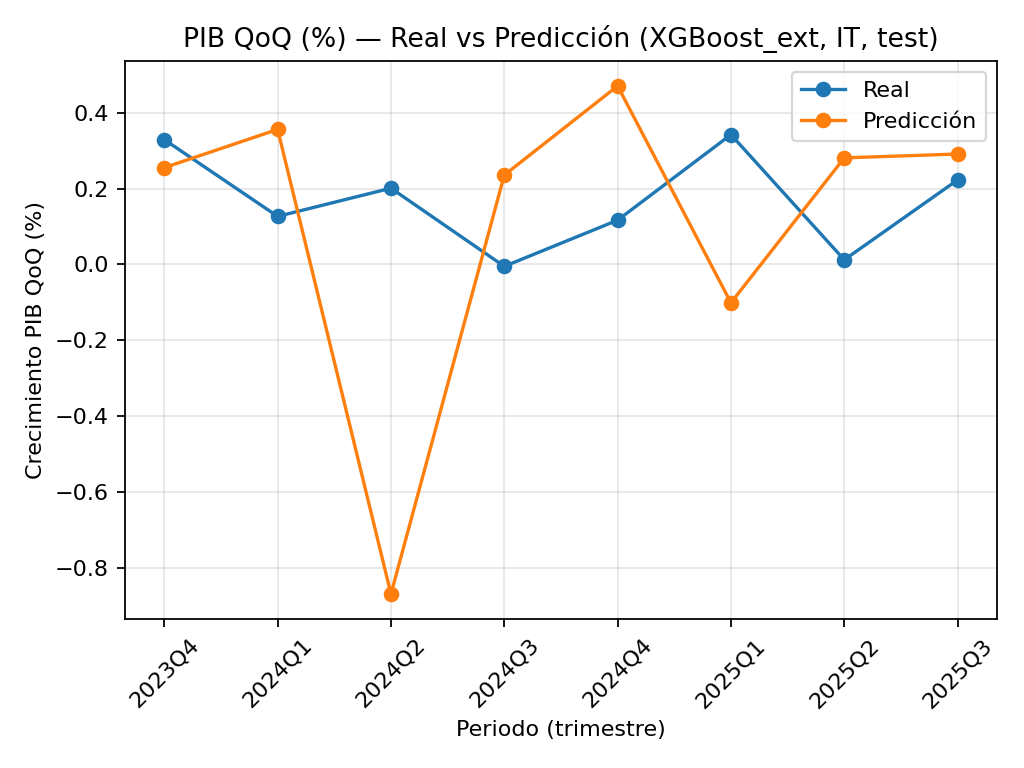
\includegraphics[width=\textwidth]{figures/bloque 0/xgboost_ext_it_real_vs_pred.png}
    \caption{PIB QoQ real vs predicción -- XGBoost ampliado (IT, test)}
    \label{fig:xgb_ext_it}
\end{minipage}
\end{figure}

\FloatBarrier
\subsection{Importancia de variables}

Las Figuras~\ref{fig:feat_es}, \ref{fig:feat_fr} y~\ref{fig:feat_it} muestran la importancia relativa de las variables según el criterio de ganancia (\textit{gain}) del modelo ampliado para cada país. En los tres casos el retardo inmediato del PIB (\texttt{gdp\_\allowbreak{}qoq\_\allowbreak{}pct\_\allowbreak{}l1}) concentra la mayor parte de la importancia explicativa, seguido a distancia por el índice de producción industrial y el comercio minorista. El desempleo y la inflación rezagados presentan una contribución marginal en los tres países, lo que sugiere que su capacidad predictiva a un trimestre vista es limitada en el periodo analizado.

\begin{figure}[H]
\centering
\begin{minipage}[t]{0.48\textwidth}
    \centering
    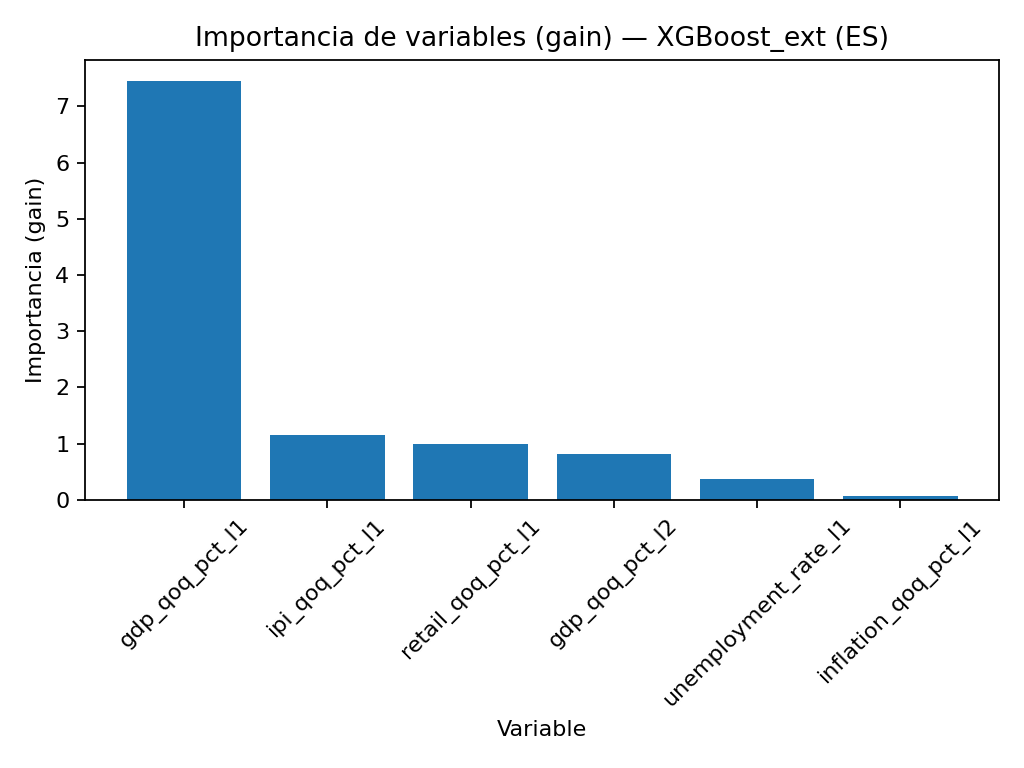
\includegraphics[width=\textwidth]{figures/bloque 0/xgboost_ext_es_feature_importance.png}
    \caption{Importancia de variables (gain) -- XGBoost ampliado (ES)}
    \label{fig:feat_es}
\end{minipage}\hfill
\begin{minipage}[t]{0.48\textwidth}
    \centering
    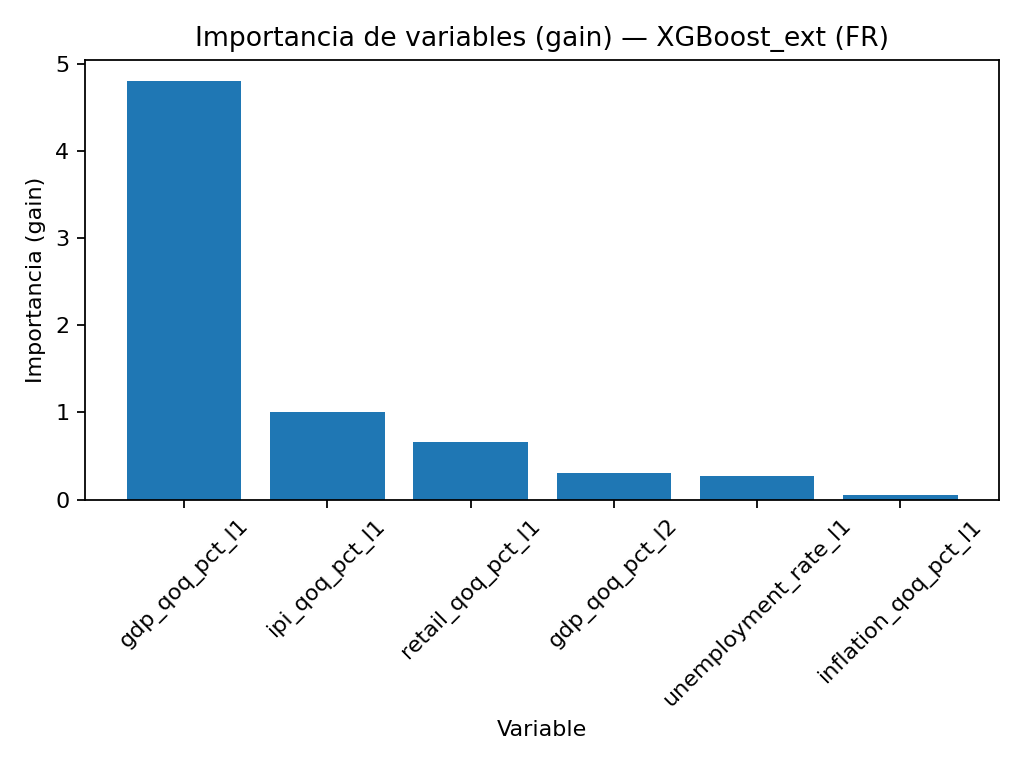
\includegraphics[width=\textwidth]{figures/bloque 0/xgboost_ext_fr_feature_importance.png}
    \caption{Importancia de variables (gain) -- XGBoost ampliado (FR)}
    \label{fig:feat_fr}
\end{minipage}
\end{figure}

\begin{figure}[H]
\centering
\begin{minipage}[t]{0.48\textwidth}
    \centering
    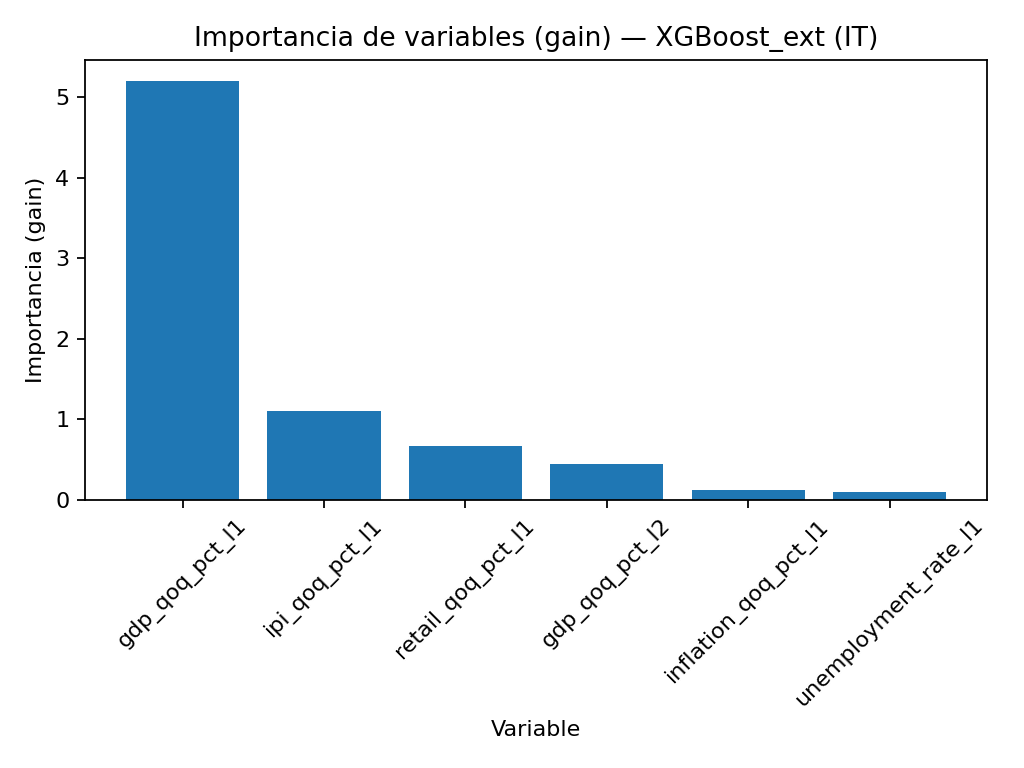
\includegraphics[width=\textwidth]{figures/bloque 0/xgboost_ext_it_feature_importance.png}
    \caption{Importancia de variables (gain) -- XGBoost ampliado (IT)}
    \label{fig:feat_it}
\end{minipage}
\end{figure}

\FloatBarrier
\subsection{Síntesis del Bloque 0}

El análisis por país revela que no existe un modelo universalmente mejor: la configuración óptima depende de la economía analizada. En España, el modelo base ofrece un mejor equilibrio entre simplicidad y capacidad de generalización, mientras que Francia e Italia se benefician de la incorporación de variables adicionales.

Este resultado sugiere que la dinámica del crecimiento económico español presenta una componente autorregresiva más débil en el periodo de prueba, de modo que añadir los retardos del propio PIB no aporta información útil y aumenta el riesgo de sobreajuste. En cambio, para Francia e Italia la incorporación de los retardos del PIB y de los indicadores de actividad económica sí mejora la capacidad predictiva, lo que indica que la dinámica de estas economías es más persistente o que los indicadores de actividad adelantan mejor el crecimiento futuro.

Adicionalmente, se observa una diferencia notable en la dificultad de predicción entre países con el modelo base: España presenta el error más bajo (MAE 0.314), seguida de Francia (0.441) e Italia (0.761), lo que apunta a diferencias estructurales en la predictibilidad del ciclo económico de cada país. Estos resultados motivan la exploración de estrategias que combinen información de múltiples países, abordada en los bloques experimentales siguientes.

% ══════════════════════════════════════════════════════════════════════
\FloatBarrier
\section{Bloque 1 --- Modelo panel combinado}

\textbf{Idea principal:} combinar los datos de los tres países en un único modelo parece reducir el sobreajuste observado en el Bloque~0, siendo el efecto más llamativo la recuperación del modelo ampliado para España (de MAE 0.796 a 0.297). El modelo panel ampliado parece ser la configuración más robusta del bloque, obteniendo resultados competitivos en los tres países de forma simultánea.

El segundo bloque de experimentos entrena un único modelo XGBoost utilizando los datos de los tres países de forma conjunta, evaluando posteriormente el rendimiento de forma separada para cada economía. A diferencia del Bloque~0, donde cada modelo solo disponía de las observaciones de su propio país (aproximadamente 58 trimestres por economía), aquí el modelo de entrenamiento accede a las ~174 observaciones combinadas del panel completo.

El objetivo de este enfoque es doble. Por un lado, aumentar el volumen de datos de entrenamiento para reducir el riesgo de sobreajuste, problema que afectó especialmente al modelo ampliado de España en el Bloque~0. Por otro, comprobar si los patrones macroeconómicos son suficientemente comunes entre las tres economías como para que un modelo compartido generalice mejor que tres modelos independientes.

Los resultados obtenidos en el conjunto de prueba son los siguientes:

\begin{table}[H]
\centering
\caption{Comparativa de modelos panel combinado por país -- Bloque 1}
\label{tab:bloque1}
\small
\begin{tabular}{lcccccc}
\hline
 & \multicolumn{2}{c}{\textbf{España}} & \multicolumn{2}{c}{\textbf{Francia}} & \multicolumn{2}{c}{\textbf{Italia}} \\
\textbf{Modelo} & \textbf{MAE} & \textbf{RMSE} & \textbf{MAE} & \textbf{RMSE} & \textbf{MAE} & \textbf{RMSE} \\
\hline
panel\_combined\_base & 0.363 & 0.462 & 0.316 & 0.426 & 0.631 & 1.039 \\
panel\_combined\_ext  & 0.297 & 0.331 & 0.215 & 0.256 & 0.376 & 0.466 \\
\hline
\end{tabular}
\end{table}

Comparando con los resultados del Bloque~0 (Tabla~\ref{tab:bloque0}), el modelo panel muestra mejoras generalizadas en el modelo ampliado y un comportamiento más consistente entre países, como se analiza en las subsecciones siguientes.

\FloatBarrier
\subsection{España}

España es el país donde el cambio de estrategia produce el impacto más destacado. El modelo ampliado, que en el Bloque~0 presentaba el peor resultado para esta economía (MAE 0.796) debido a una predicción anómala de $-2.5$ p.p. en 2023Q4, pasa ahora a obtener el mejor resultado con MAE 0.297, superando incluso al modelo base del panel (MAE 0.363).

Este resultado apunta al efecto regularizador del mayor volumen de datos: al entrenar con las observaciones combinadas de los tres países, el modelo ampliado parece dejar de memorizar los retardos del PIB español y adquiere una mayor capacidad de generalización. Las Figuras~\ref{fig:panel_base_es_pred} y~\ref{fig:panel_ext_es_pred} permiten apreciar visualmente esta mejora. El modelo base del panel (Figura~\ref{fig:panel_base_es_pred}) sigue con dificultad la aceleración del crecimiento español en 2024Q1 y tiende a subestimar los trimestres finales del periodo de prueba. El modelo ampliado del panel (Figura~\ref{fig:panel_ext_es_pred}), en cambio, captura mejor la tendencia general, aunque sobreestima el pico de 2024Q3 y no anticipa la moderación posterior.

Los errores de predicción, representados en las Figuras~\ref{fig:panel_base_es_err} y~\ref{fig:panel_ext_es_err}, muestran que ambos modelos producen errores de signo variable sin un sesgo sistemático claro. El modelo ampliado presenta errores más contenidos y distribuidos de forma más homogénea a lo largo del periodo de prueba, mientras que el modelo base acumula errores positivos crecientes hacia el final del horizonte.

\begin{figure}[H]
\centering
\begin{minipage}[t]{0.48\textwidth}
    \centering
    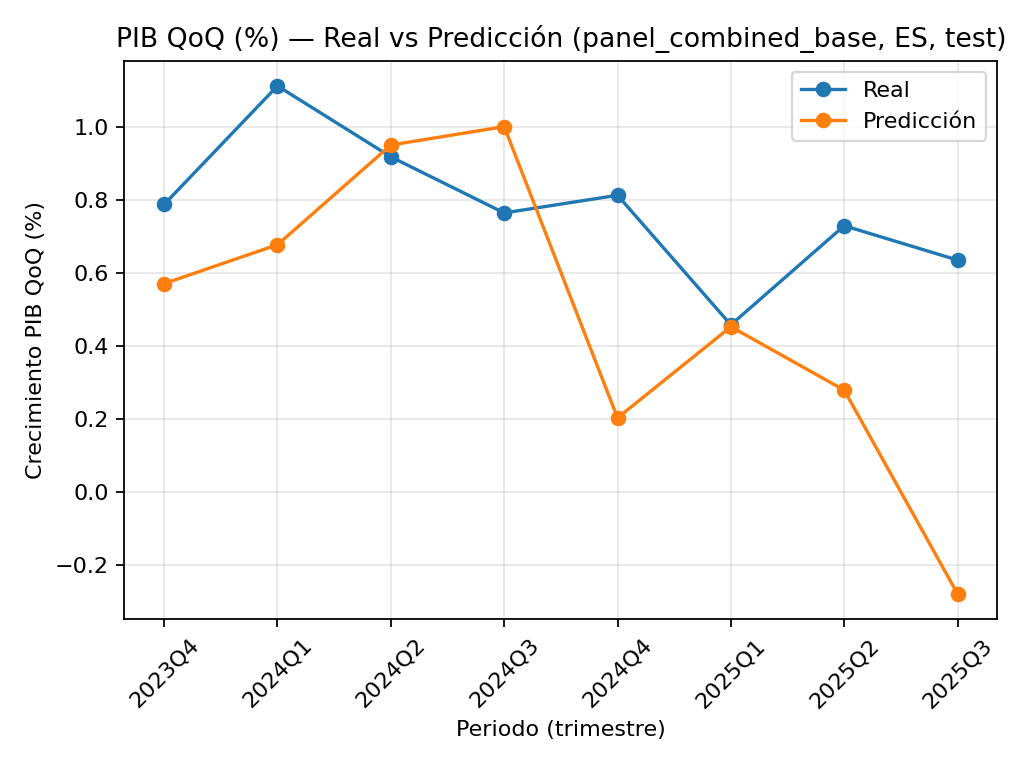
\includegraphics[width=\textwidth]{figures/bloque 1/panel_combined_base_es_real_vs_pred.png}
    \caption{PIB QoQ real vs predicción -- panel combinado base (ES, test)}
    \label{fig:panel_base_es_pred}
\end{minipage}\hfill
\begin{minipage}[t]{0.48\textwidth}
    \centering
    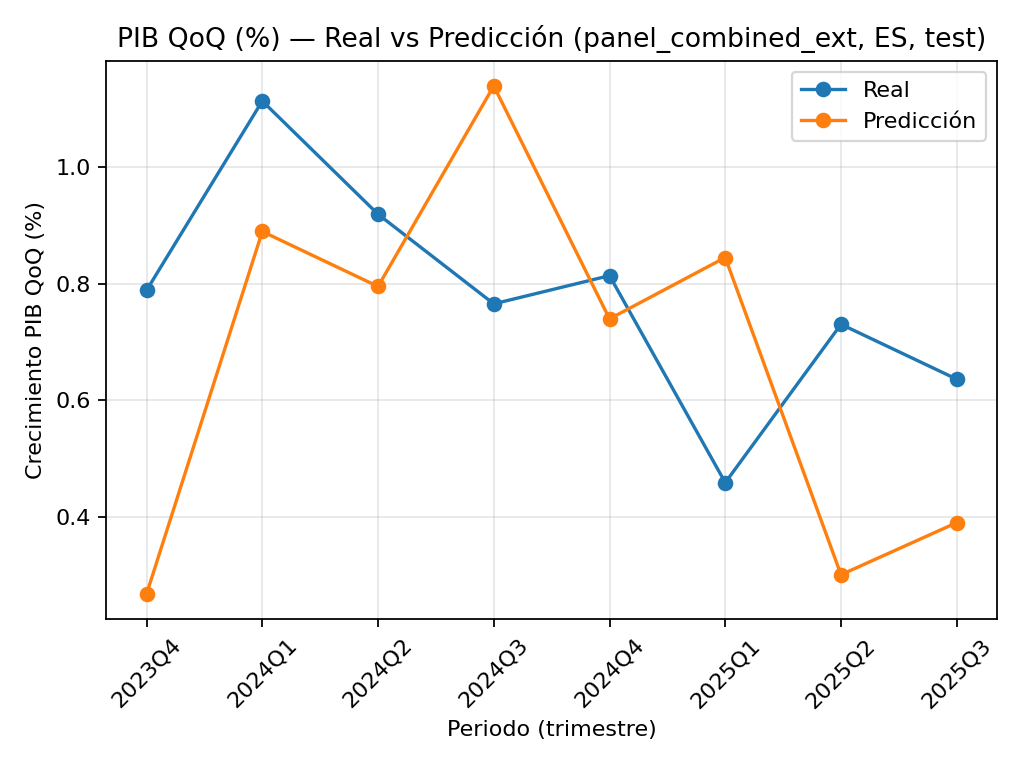
\includegraphics[width=\textwidth]{figures/bloque 1/panel_combined_ext_es_real_vs_pred.png}
    \caption{PIB QoQ real vs predicción -- panel combinado ampliado (ES, test)}
    \label{fig:panel_ext_es_pred}
\end{minipage}

\vspace{0.5em}

\begin{minipage}[t]{0.48\textwidth}
    \centering
    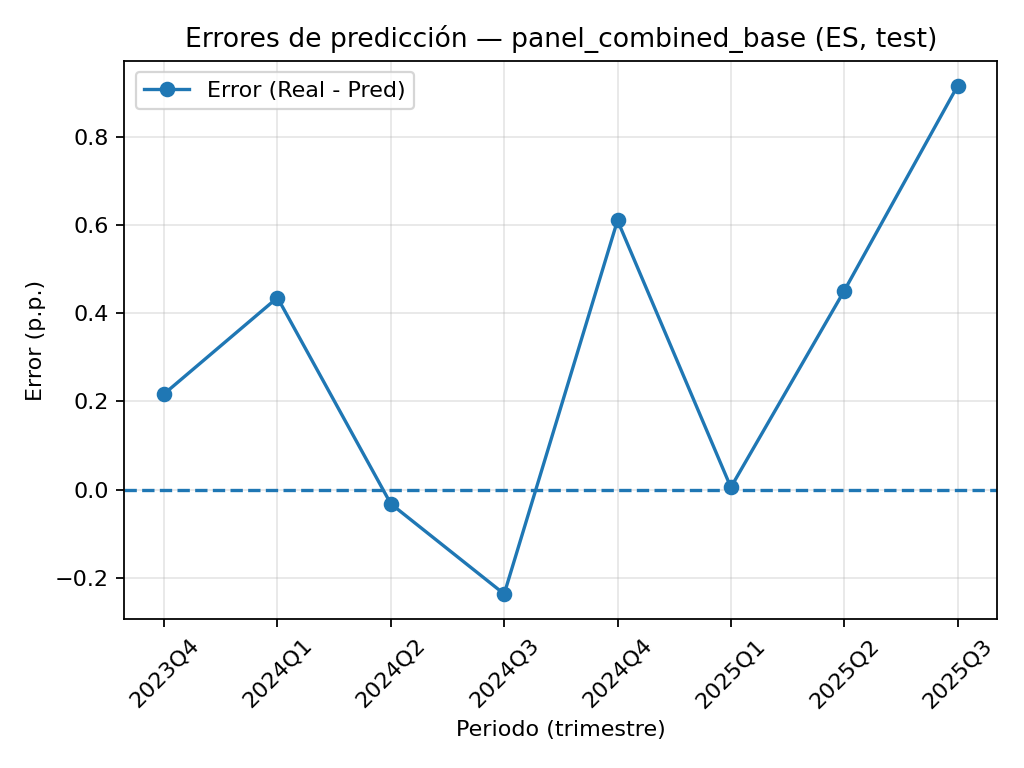
\includegraphics[width=\textwidth]{figures/bloque 1/panel_combined_base_es_errors.png}
    \caption{Errores de predicción -- panel combinado base (ES, test)}
    \label{fig:panel_base_es_err}
\end{minipage}\hfill
\begin{minipage}[t]{0.48\textwidth}
    \centering
    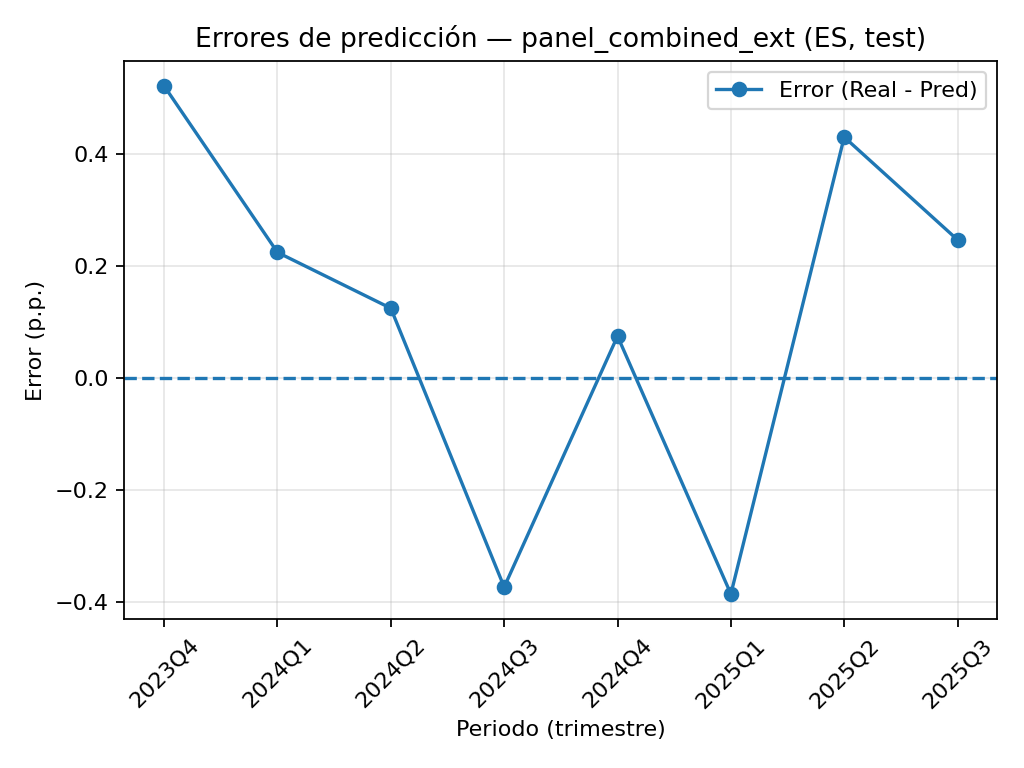
\includegraphics[width=\textwidth]{figures/bloque 1/panel_combined_ext_es_errors.png}
    \caption{Errores de predicción -- panel combinado ampliado (ES, test)}
    \label{fig:panel_ext_es_err}
\end{minipage}
\end{figure}

\FloatBarrier
\subsection{Francia}

Francia confirma los buenos resultados ya obtenidos en el Bloque~0 y los mejora en ambas configuraciones. El modelo ampliado reduce su MAE de 0.193 a 0.215 --- una diferencia mínima que puede atribuirse a variabilidad muestral ---, mientras que el modelo base mejora notablemente, pasando de MAE 0.441 a 0.316. Este resultado indica que el panel conjunto es especialmente beneficioso para la configuración base, que en el Bloque~0 carecía de suficiente señal predictiva con solo dos variables y los datos de un único país.

La Figura~\ref{fig:panel_base_fr_pred} muestra que el modelo base del panel ya no oscila de forma tan pronunciada como en el Bloque~0, sino que sigue con mayor suavidad la evolución real del crecimiento francés. El modelo ampliado (Figura~\ref{fig:panel_ext_fr_pred}) mantiene un ajuste similar al del Bloque~0, con una sobreestimación moderada en 2024Q3 y cierta dificultad para anticipar la caída de 2024Q4, aunque las magnitudes de error son en general contenidas.

Los gráficos de error de las Figuras~\ref{fig:panel_base_fr_err} y~\ref{fig:panel_ext_fr_err} revelan que el error más pronunciado del modelo base se concentra en 2024Q3, donde la predicción se aleja aproximadamente 0.94 p.p. del valor real. El modelo ampliado distribuye mejor los errores a lo largo del periodo, con valores que raramente superan $\pm 0.45$ p.p.

\begin{figure}[H]
\centering
\begin{minipage}[t]{0.48\textwidth}
    \centering
    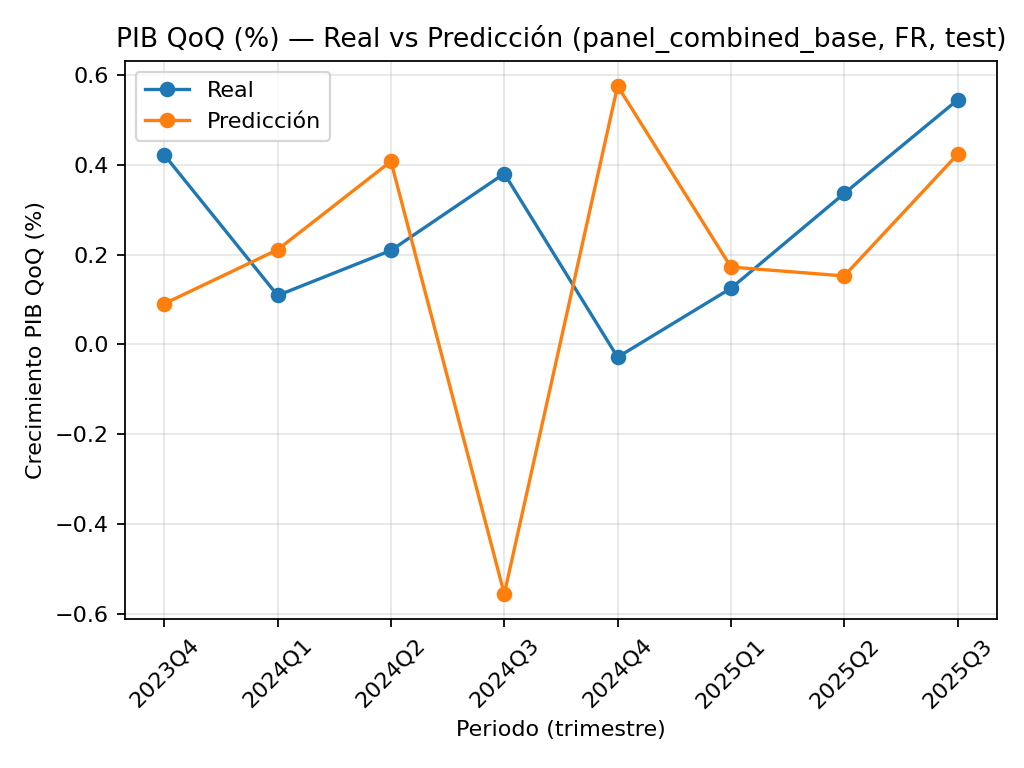
\includegraphics[width=\textwidth]{figures/bloque 1/panel_combined_base_fr_real_vs_pred.png}
    \caption{PIB QoQ real vs predicción -- panel combinado base (FR, test)}
    \label{fig:panel_base_fr_pred}
\end{minipage}\hfill
\begin{minipage}[t]{0.48\textwidth}
    \centering
    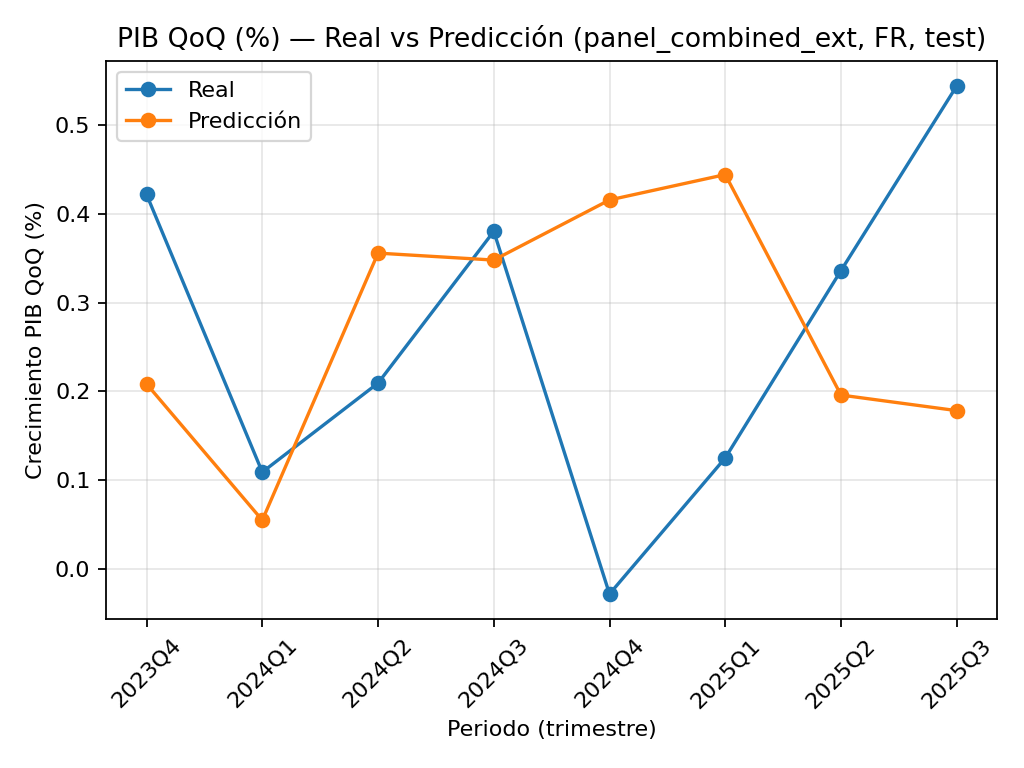
\includegraphics[width=\textwidth]{figures/bloque 1/panel_combined_ext_fr_real_vs_pred.png}
    \caption{PIB QoQ real vs predicción -- panel combinado ampliado (FR, test)}
    \label{fig:panel_ext_fr_pred}
\end{minipage}

\vspace{0.5em}

\begin{minipage}[t]{0.48\textwidth}
    \centering
    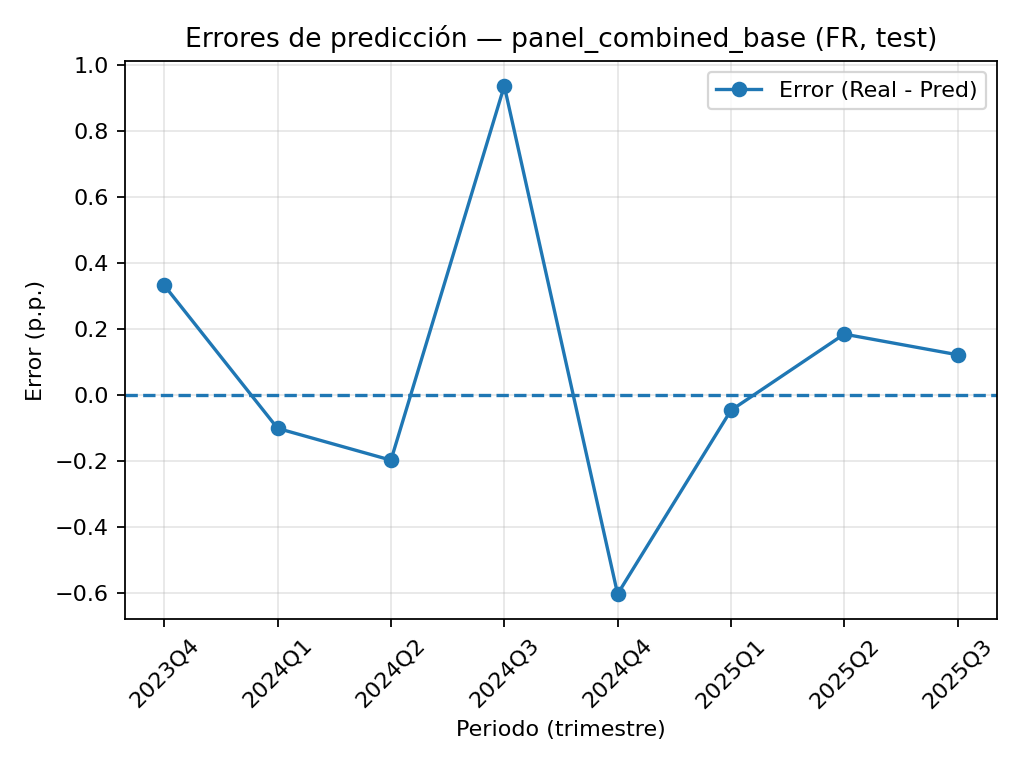
\includegraphics[width=\textwidth]{figures/bloque 1/panel_combined_base_fr_errors.png}
    \caption{Errores de predicción -- panel combinado base (FR, test)}
    \label{fig:panel_base_fr_err}
\end{minipage}\hfill
\begin{minipage}[t]{0.48\textwidth}
    \centering
    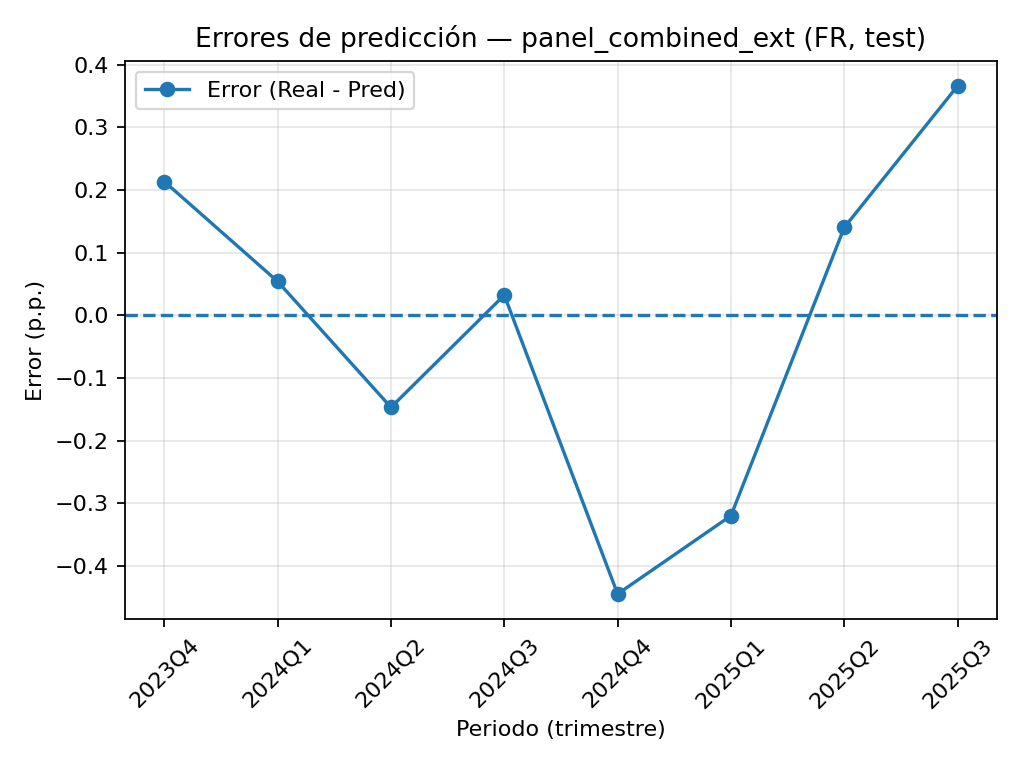
\includegraphics[width=\textwidth]{figures/bloque 1/panel_combined_ext_fr_errors.png}
    \caption{Errores de predicción -- panel combinado ampliado (FR, test)}
    \label{fig:panel_ext_fr_err}
\end{minipage}
\end{figure}

\FloatBarrier
\subsection{Italia}

Italia sigue siendo el país con mayor dificultad de predicción en ambas configuraciones. El modelo base mejora su MAE de 0.761 a 0.631 respecto al Bloque~0, aunque su RMSE asciende a 1.039, el valor más alto de todo el bloque. La gran distancia entre MAE y RMSE delata la presencia de al menos un error puntual muy elevado ---visible en los gráficos de error--- que infla el RMSE sin que el error medio sea tan llamativo. El modelo ampliado presenta un MAE de 0.376, ligeramente superior al 0.344 del Bloque~0, pero con un RMSE de 0.466 que sí mejora el 0.455 anterior, indicando que los errores extremos se han suavizado aunque el error típico haya aumentado marginalmente.

La Figura~\ref{fig:panel_base_it_pred} muestra que el modelo base del panel corrige en parte el comportamiento errático observado en el Bloque~0, donde la predicción llegó a situarse en $-0.07$ p.p. cuando el crecimiento real era de $0.34$ p.p. Aun así, las predicciones siguen sin capturar bien la variabilidad trimestral italiana, que presenta oscilaciones más bruscas que las de España o Francia. El modelo ampliado (Figura~\ref{fig:panel_ext_it_pred}) reproduce mejor la dirección general del crecimiento, aunque los gráficos de error (Figuras~\ref{fig:panel_base_it_err} y~\ref{fig:panel_ext_it_err}) revelan errores puntuales superiores a 0.8 p.p. en 2024Q1 y 2024Q4, trimestres en los que el modelo no anticipa la magnitud de los cambios en la actividad económica italiana.

\begin{figure}[H]
\centering
\begin{minipage}[t]{0.48\textwidth}
    \centering
    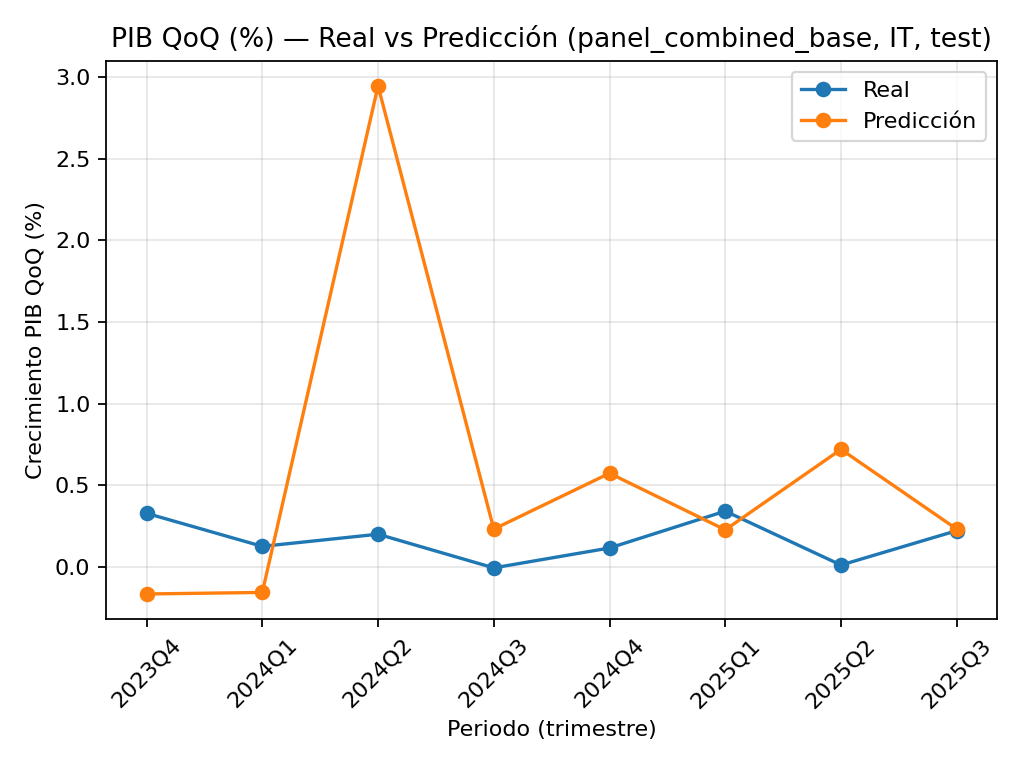
\includegraphics[width=\textwidth]{figures/bloque 1/panel_combined_base_it_real_vs_pred.png}
    \caption{PIB QoQ real vs predicción -- panel combinado base (IT, test)}
    \label{fig:panel_base_it_pred}
\end{minipage}\hfill
\begin{minipage}[t]{0.48\textwidth}
    \centering
    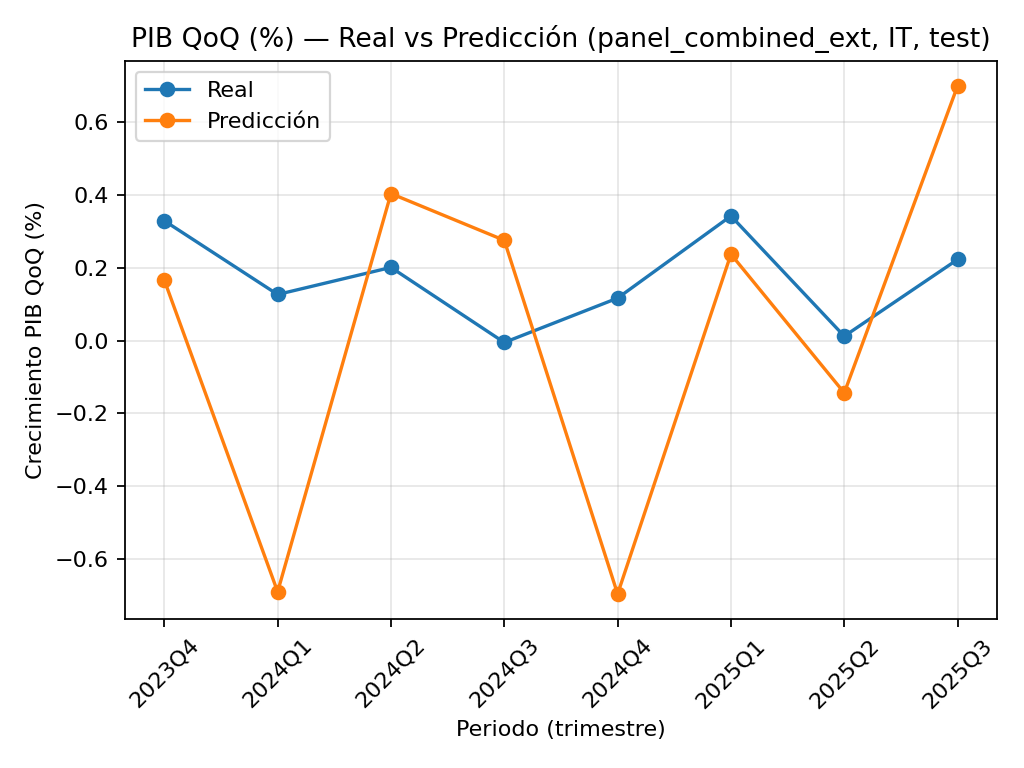
\includegraphics[width=\textwidth]{figures/bloque 1/panel_combined_ext_it_real_vs_pred.png}
    \caption{PIB QoQ real vs predicción -- panel combinado ampliado (IT, test)}
    \label{fig:panel_ext_it_pred}
\end{minipage}

\vspace{0.5em}

\begin{minipage}[t]{0.48\textwidth}
    \centering
    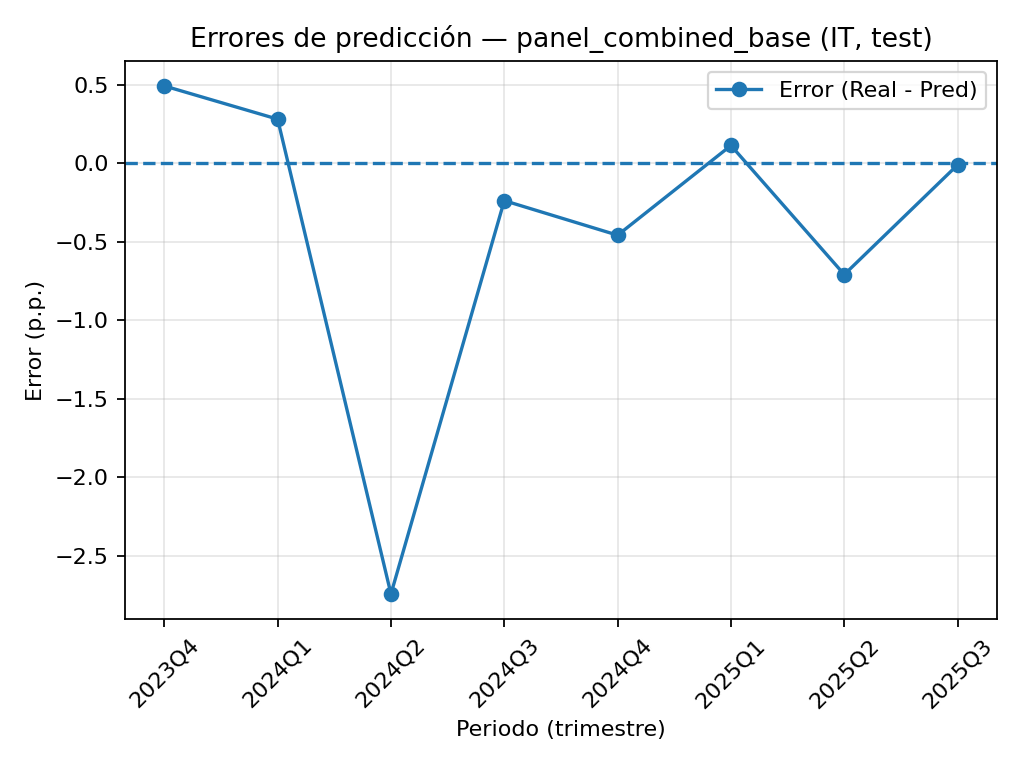
\includegraphics[width=\textwidth]{figures/bloque 1/panel_combined_base_it_errors.png}
    \caption{Errores de predicción -- panel combinado base (IT, test)}
    \label{fig:panel_base_it_err}
\end{minipage}\hfill
\begin{minipage}[t]{0.48\textwidth}
    \centering
    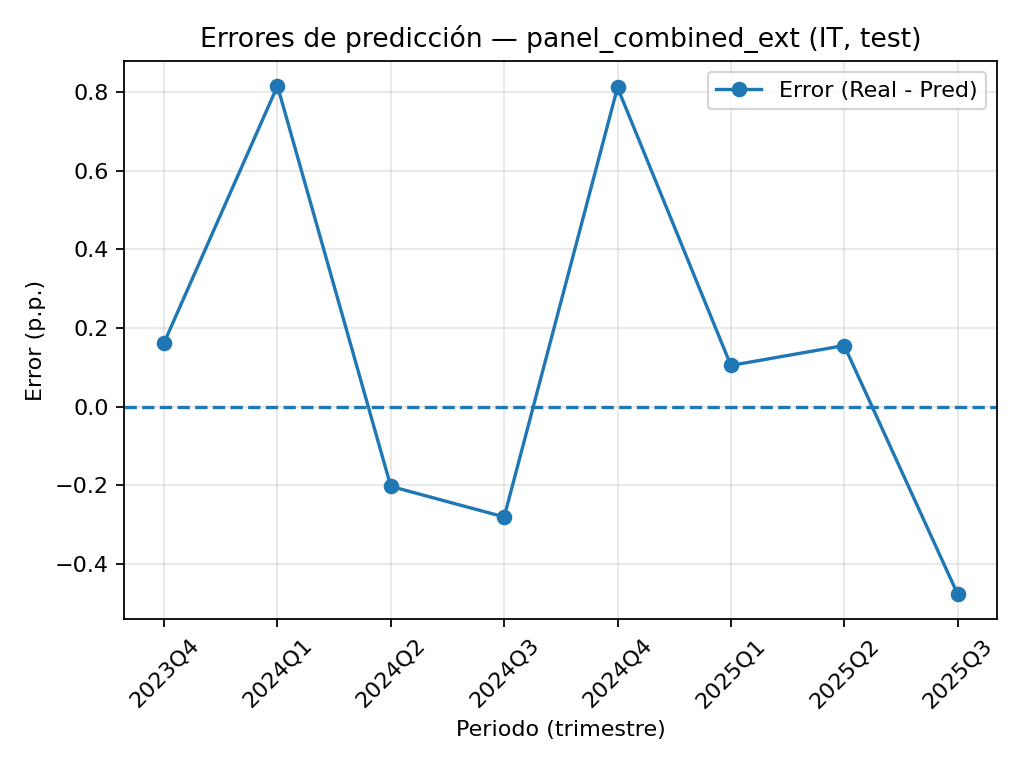
\includegraphics[width=\textwidth]{figures/bloque 1/panel_combined_ext_it_errors.png}
    \caption{Errores de predicción -- panel combinado ampliado (IT, test)}
    \label{fig:panel_ext_it_err}
\end{minipage}
\end{figure}

\FloatBarrier
\subsection{Importancia de variables}

Las Figuras~\ref{fig:panel_feat_base} y~\ref{fig:panel_feat_ext} muestran la importancia relativa de las variables en el modelo panel para las configuraciones base y ampliada respectivamente.

En el modelo base (Figura~\ref{fig:panel_feat_base}), las únicas dos variables disponibles ---inflación rezagada (\texttt{inflation\_\allowbreak{}qoq\_\allowbreak{}pct\_\allowbreak{}l1}) y tasa de desempleo rezagada (\texttt{unemployment\_\allowbreak{}rate\_\allowbreak{}l1})--- presentan una importancia relativamente equilibrada, con la inflación algo por encima (ganancia aproximada de 6.3 frente a 4.1). Este reparto contrasta con la dominancia habitual de los retardos del PIB en el modelo ampliado, y sugiere que, cuando no se dispone de información autorregresiva, ambos indicadores macroeconómicos aportan señal útil de forma complementaria.

En el modelo ampliado (Figura~\ref{fig:panel_feat_ext}), el retardo inmediato del PIB (\texttt{gdp\_\allowbreak{}qoq\_\allowbreak{}pct\_\allowbreak{}l1}) concentra de nuevo la mayor parte de la importancia explicativa (ganancia próxima a 15), reproduciendo el patrón ya observado en el Bloque~0 para los modelos por país. El índice de producción industrial (\texttt{ipi\_\allowbreak{}qoq\_\allowbreak{}pct\_\allowbreak{}l1}) y el comercio minorista (\texttt{retail\_\allowbreak{}qoq\_\allowbreak{}pct\_\allowbreak{}l1}) ocupan el segundo y tercer lugar respectivamente, con ganancias en torno a 2.5 y 2.0. El desempleo y la inflación rezagados mantienen una contribución marginal, lo que confirma que, una vez disponibles los retardos del PIB y los indicadores de actividad, las variables de mercado laboral y precios no añaden capacidad predictiva adicional a un horizonte de un trimestre.

\begin{figure}[H]
\centering
\begin{minipage}[t]{0.48\textwidth}
    \centering
    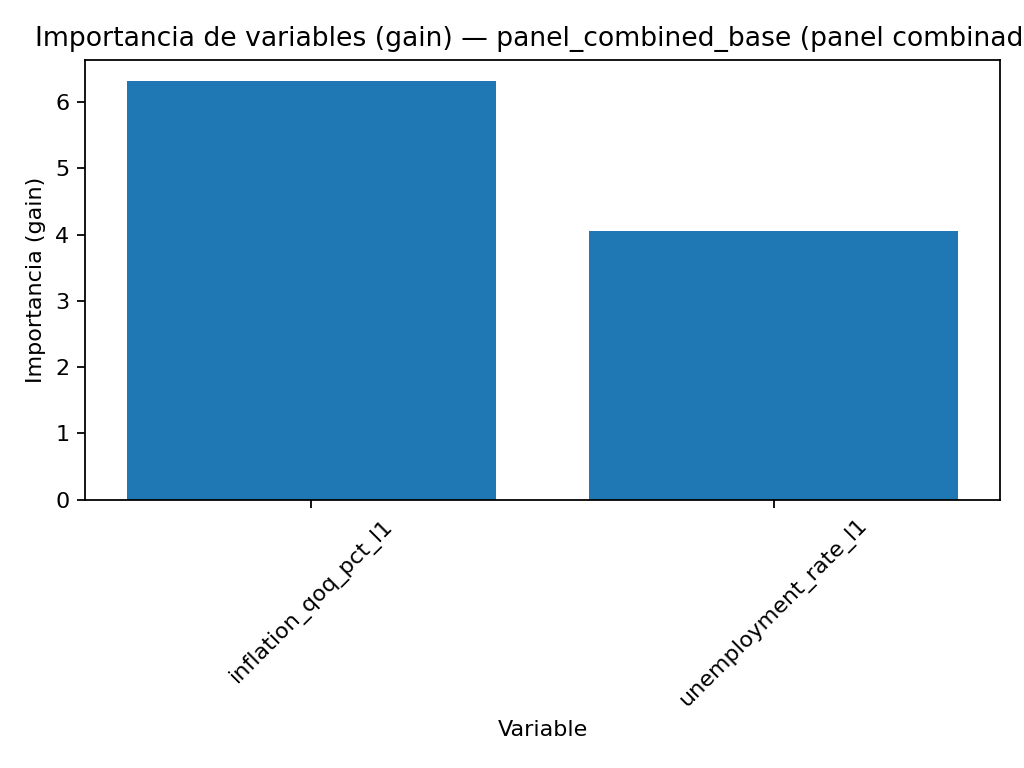
\includegraphics[width=\textwidth]{figures/bloque 1/panel_combined_base_combined_feature_importance.png}
    \caption{Importancia de variables (gain) -- panel combinado base}
    \label{fig:panel_feat_base}
\end{minipage}\hfill
\begin{minipage}[t]{0.48\textwidth}
    \centering
    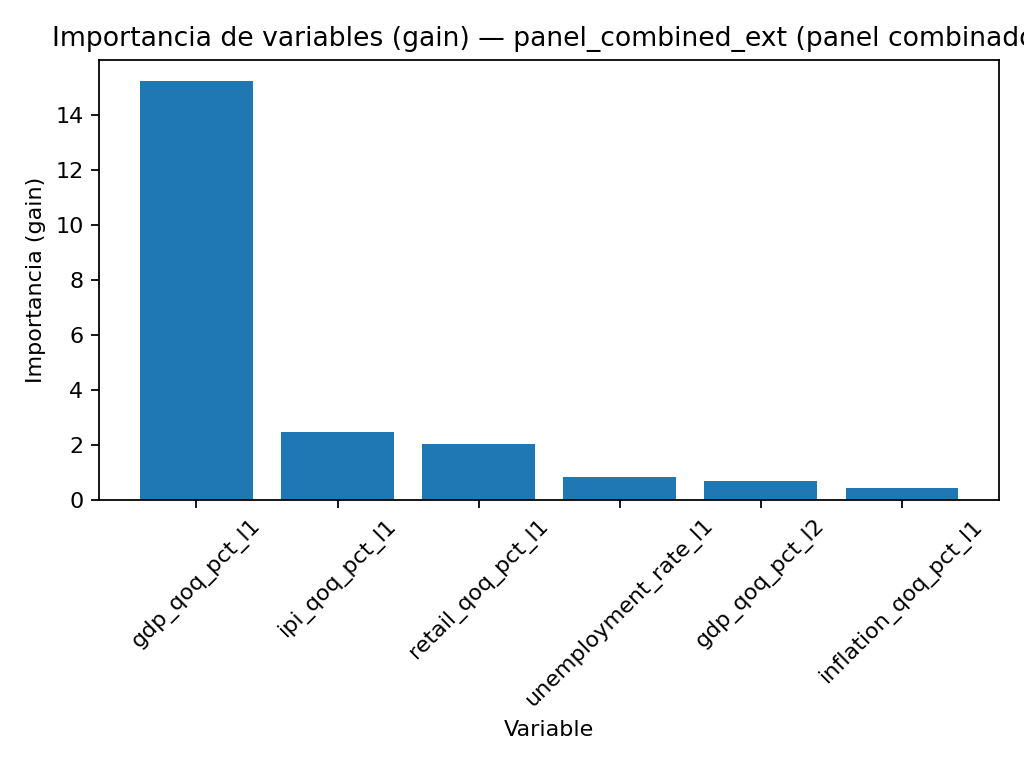
\includegraphics[width=\textwidth]{figures/bloque 1/panel_combined_ext_combined_feature_importance.png}
    \caption{Importancia de variables (gain) -- panel combinado ampliado}
    \label{fig:panel_feat_ext}
\end{minipage}
\end{figure}

\FloatBarrier
\subsection{Síntesis del Bloque 1}

El entrenamiento con datos combinados de los tres países produce mejoras generalizadas respecto al Bloque~0, siendo el efecto más significativo la rehabilitación del modelo ampliado para España, que pasa de ser el peor resultado individual (MAE 0.796) al mejor del bloque (MAE 0.297). Este resultado sugiere que el sobreajuste observado en el Bloque~0 podría estar relacionado principalmente con la escasez de datos de entrenamiento, más que con una limitación inherente de las variables seleccionadas.

Desde una perspectiva metodológica, el modelo panel ampliado se consolida como la configuración más robusta del bloque: obtiene el mejor MAE en los tres países de forma simultánea, algo que ninguna configuración del Bloque~0 lograba. La tabla comparativa entre bloques ilustra esta consistencia: frente a la heterogeneidad de resultados del Bloque~0 ---donde la configuración óptima variaba según el país---, el modelo panel ampliado ofrece un resultado competitivo de forma uniforme.

Italia sigue siendo el país más difícil de predecir, con un MAE del modelo ampliado (0.376) que duplica aproximadamente el de España (0.297) y supera al de Francia (0.215). Esto apunta a que la economía italiana presenta una dinámica trimestral menos persistente o más sensible a factores no capturados por las variables del panel, lo que motiva la exploración de enfoques que permitan al modelo distinguir explícitamente entre economías, abordada en el Bloque~2.

% ══════════════════════════════════════════════════════════════════════
\FloatBarrier
\section{Bloque 2 --- Panel con variable \emph{geo} como feature}

\textbf{Idea principal:} incorporar dummies de país resulta beneficioso únicamente cuando el modelo ya dispone de variables autorregresivas. Sin ellas, las dummies parecen sobreexplotarse y degradan gravemente las predicciones ---con un colapso extremo en Italia (MAE 4.324)---. El modelo ampliado con geo obtiene resultados similares o ligeramente superiores a los del Bloque~1.

El tercer bloque de experimentos parte de la misma arquitectura del Bloque~1 pero introduce
una modificación conceptualmente relevante: la variable de país se incorpora explícitamente
como feature mediante codificación \emph{one-hot}, añadiendo tres columnas binarias
(\texttt{geo\_ES}, \texttt{geo\_FR}, \texttt{geo\_IT}) al vector de entrada del modelo.

En el Bloque~1, el modelo panel compartía todos sus parámetros sin distinguir la procedencia
de cada observación; el único mecanismo de diferenciación era indirecto, a través de las
diferencias en los valores de los indicadores macroeconómicos entre países. El Bloque~2
permite que el modelo aprenda umbrales y reglas distintos para cada economía sin necesidad
de entrenar modelos separados.

El dataset, la partición temporal, los hiperparámetros del modelo XGBoost y las dos
configuraciones de features (base y ampliada) son idénticos a los bloques anteriores.
La única diferencia es la adición de \texttt{geo\_ES}, \texttt{geo\_FR} y \texttt{geo\_IT}
al final del vector de entrada en ambas configuraciones, elevando el número de features
de 2 a 5 en el modelo base, y de 6 a 9 en el modelo ampliado.

Los resultados obtenidos en el conjunto de prueba para los tres países son los siguientes:

\begin{table}[H]
\centering
\caption{Comparativa de modelos panel con geo como feature por país -- Bloque 2}
\label{tab:bloque2}
\small
\begin{tabular}{lcccccc}
\hline
 & \multicolumn{2}{c}{\textbf{España}} & \multicolumn{2}{c}{\textbf{Francia}} & \multicolumn{2}{c}{\textbf{Italia}} \\
\textbf{Modelo} & \textbf{MAE} & \textbf{RMSE} & \textbf{MAE} & \textbf{RMSE} & \textbf{MAE} & \textbf{RMSE} \\
\hline
panel\_geo\_base & 0.423 & 0.466 & 0.819 & 1.021 & 4.324 & 6.518 \\
panel\_geo\_ext  & 0.290 & 0.331 & 0.224 & 0.270 & 0.365 & 0.451 \\
\hline
\end{tabular}
\end{table}

El contraste entre ambas configuraciones es el más acusado de todos los bloques analizados:
el modelo base con dummies de país registra resultados muy inferiores a los del Bloque~1,
mientras que el modelo ampliado mantiene o mejora marginalmente los resultados previos.

\FloatBarrier
\subsection{España}

Para España, el modelo base del panel geo obtiene un MAE de 0.423, superior a los 0.363 del
Bloque~1. Como muestra la Figura~\ref{fig:b2_base_es_pred}, el modelo subestima de forma
sistemática el crecimiento en los primeros trimestres del horizonte de prueba y sobreestima
bruscamente en 2024Q3, para finalmente caer a territorio negativo en 2025Q3 cuando la
economía española aún crecía 0.64~p.p. El gráfico de errores
(Figura~\ref{fig:b2_base_es_err}) refleja esta inestabilidad con una alternancia de signo
pronunciada que supera los $\pm$0.6~p.p. en varios trimestres.

El modelo ampliado obtiene un MAE de 0.290, su mejor resultado en todos los bloques para
España, con una mejora marginal respecto a los 0.297 del Bloque~1. La
Figura~\ref{fig:b2_ext_es_pred} muestra que las dos curvas evolucionan de forma muy similar,
sin llegar a producir ninguna predicción anómala. El gráfico de errores
(Figura~\ref{fig:b2_ext_es_err}) no presenta sesgo sistemático, con valores que oscilan
entre $-$0.29 y 0.55~p.p.

\begin{figure}[H]
\centering
\begin{minipage}[t]{0.48\textwidth}
    \centering
    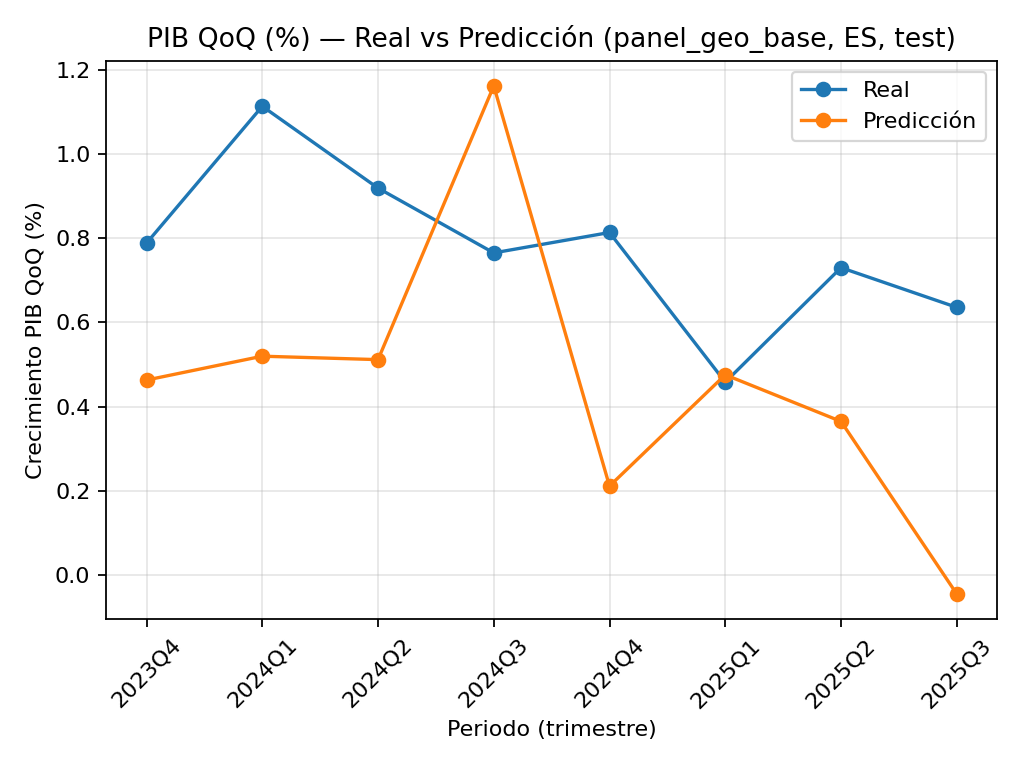
\includegraphics[width=\textwidth]{figures/bloque 2/panel_geo_base_es_real_vs_pred.png}
    \caption{PIB QoQ real vs predicción -- panel geo base (ES, test)}
    \label{fig:b2_base_es_pred}
\end{minipage}\hfill
\begin{minipage}[t]{0.48\textwidth}
    \centering
    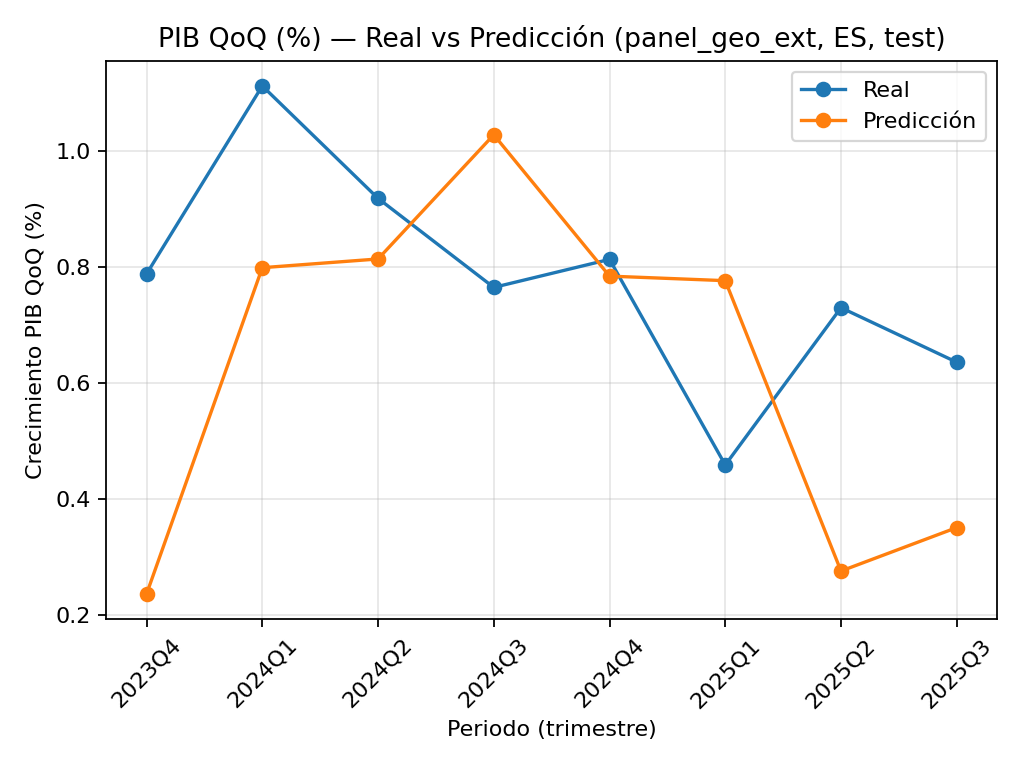
\includegraphics[width=\textwidth]{figures/bloque 2/panel_geo_ext_es_real_vs_pred.png}
    \caption{PIB QoQ real vs predicción -- panel geo ampliado (ES, test)}
    \label{fig:b2_ext_es_pred}
\end{minipage}

\vspace{0.5em}

\begin{minipage}[t]{0.48\textwidth}
    \centering
    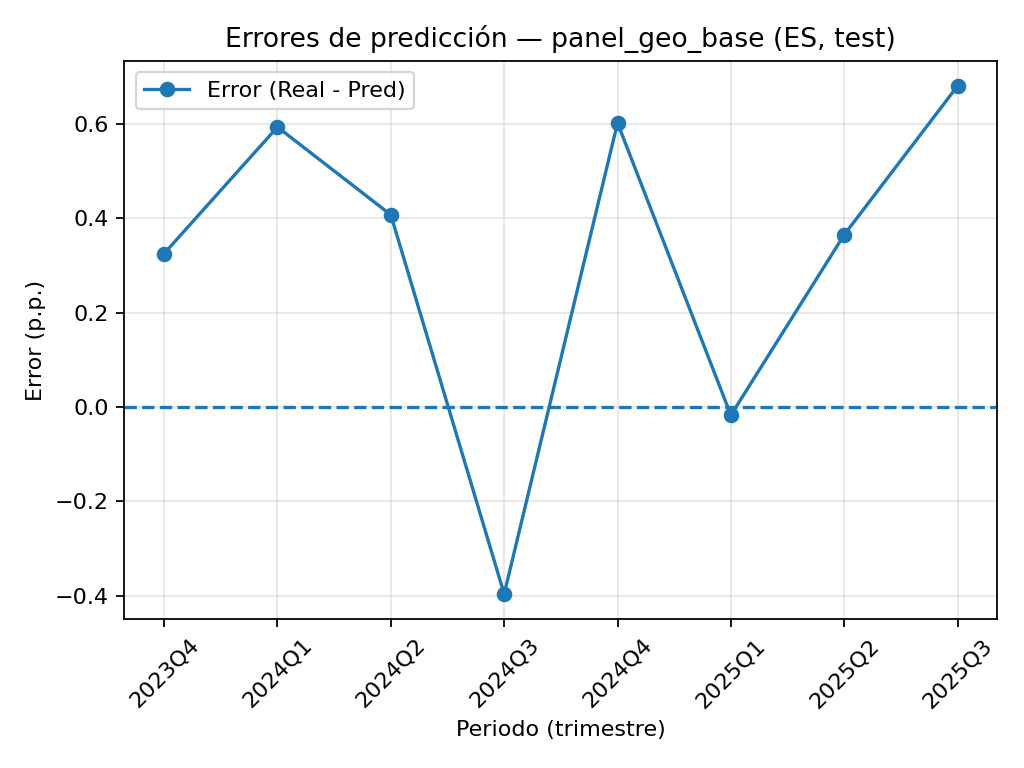
\includegraphics[width=\textwidth]{figures/bloque 2/panel_geo_base_es_errors.png}
    \caption{Errores de predicción -- panel geo base (ES, test)}
    \label{fig:b2_base_es_err}
\end{minipage}\hfill
\begin{minipage}[t]{0.48\textwidth}
    \centering
    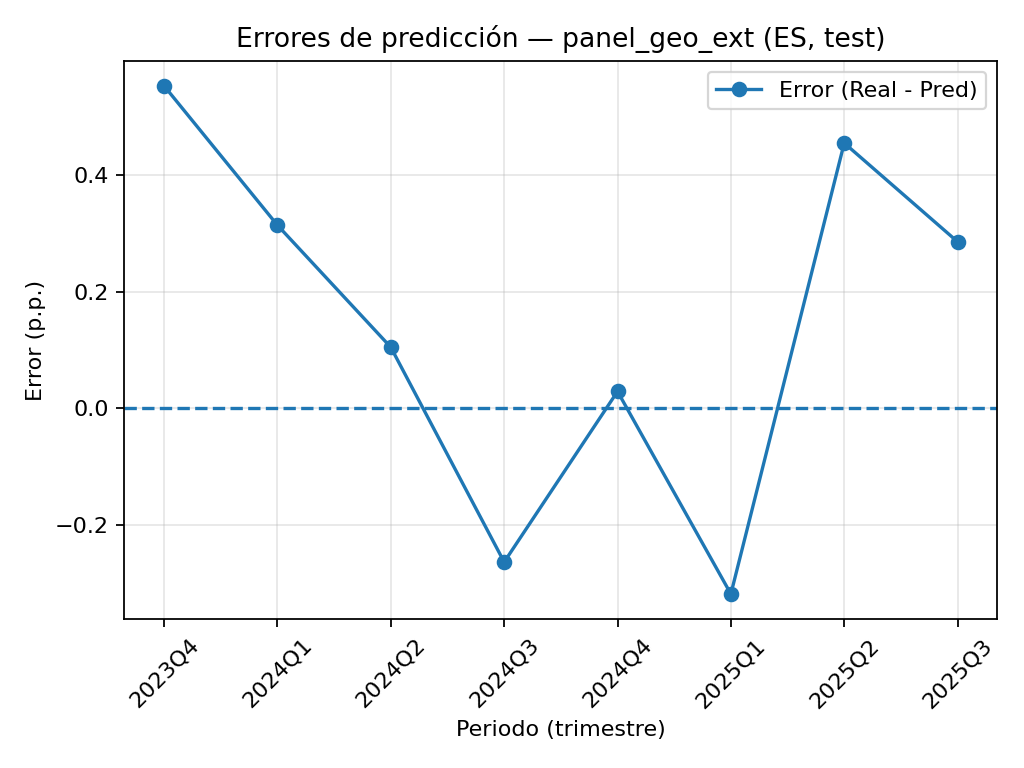
\includegraphics[width=\textwidth]{figures/bloque 2/panel_geo_ext_es_errors.png}
    \caption{Errores de predicción -- panel geo ampliado (ES, test)}
    \label{fig:b2_ext_es_err}
\end{minipage}
\end{figure}

\FloatBarrier
\subsection{Francia}

Francia es el país donde la introducción de las dummies de país produce el deterioro más
severo en la configuración base, pasando de un MAE de 0.316 en el Bloque~1 a 0.819 en el
Bloque~2. La Figura~\ref{fig:b2_base_fr_pred} ilustra el problema de forma inequívoca:
mientras que el crecimiento real de Francia se mantiene en un rango estrecho a lo largo del
periodo de prueba, las predicciones oscilan violentamente, con errores que alcanzan valores
inferiores a $-$1.5~p.p. en varios trimestres de 2025
(Figura~\ref{fig:b2_base_fr_err}). Este comportamiento se explica porque, sin los retardos
del PIB que anclen las predicciones al nivel de actividad reciente, la dummy
\texttt{geo\_FR} lleva al modelo a activar regiones del espacio de features asociadas en el
entrenamiento a trimestres de alto crecimiento francés que no vuelven a reproducirse en el
periodo de prueba.

El modelo ampliado recupera la capacidad predictiva con un MAE de 0.224, apenas
0.009~p.p. superior al 0.215 del Bloque~1, diferencia que se sitúa dentro de la variabilidad
esperada con solo 8 observaciones de prueba. La Figura~\ref{fig:b2_ext_fr_pred} muestra que
la predicción sigue la evolución real con razonable fidelidad, con errores contenidos en la
mayor parte del periodo (Figura~\ref{fig:b2_ext_fr_err}).

\begin{figure}[H]
\centering
\begin{minipage}[t]{0.48\textwidth}
    \centering
    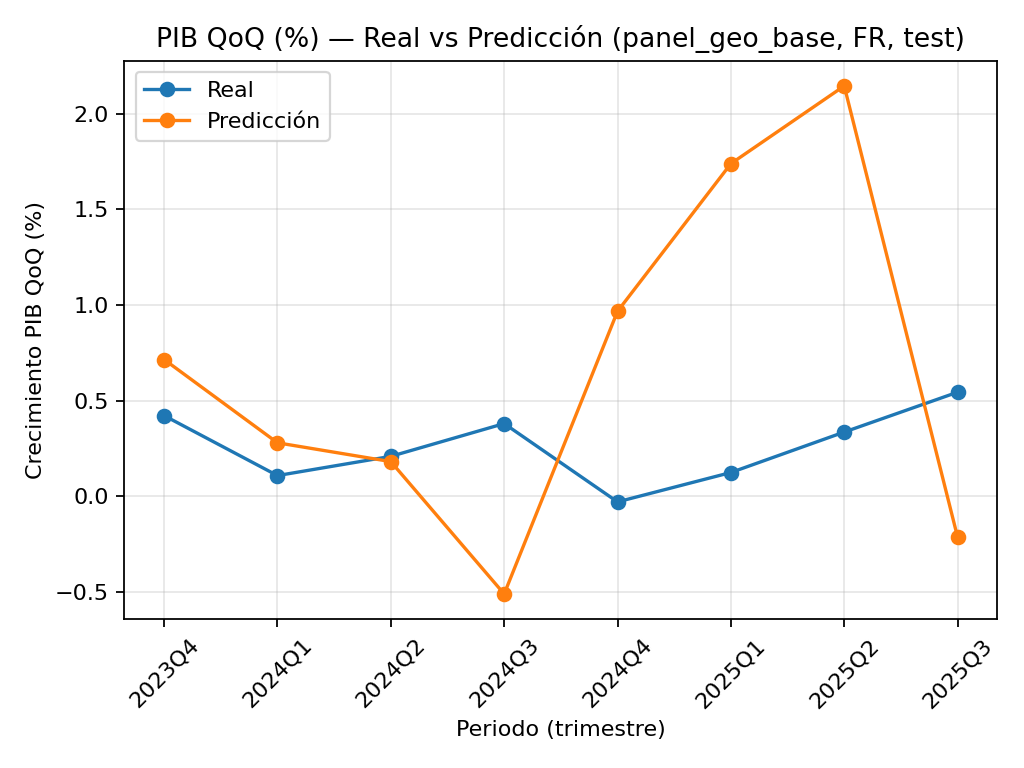
\includegraphics[width=\textwidth]{figures/bloque 2/panel_geo_base_fr_real_vs_pred.png}
    \caption{PIB QoQ real vs predicción -- panel geo base (FR, test)}
    \label{fig:b2_base_fr_pred}
\end{minipage}\hfill
\begin{minipage}[t]{0.48\textwidth}
    \centering
    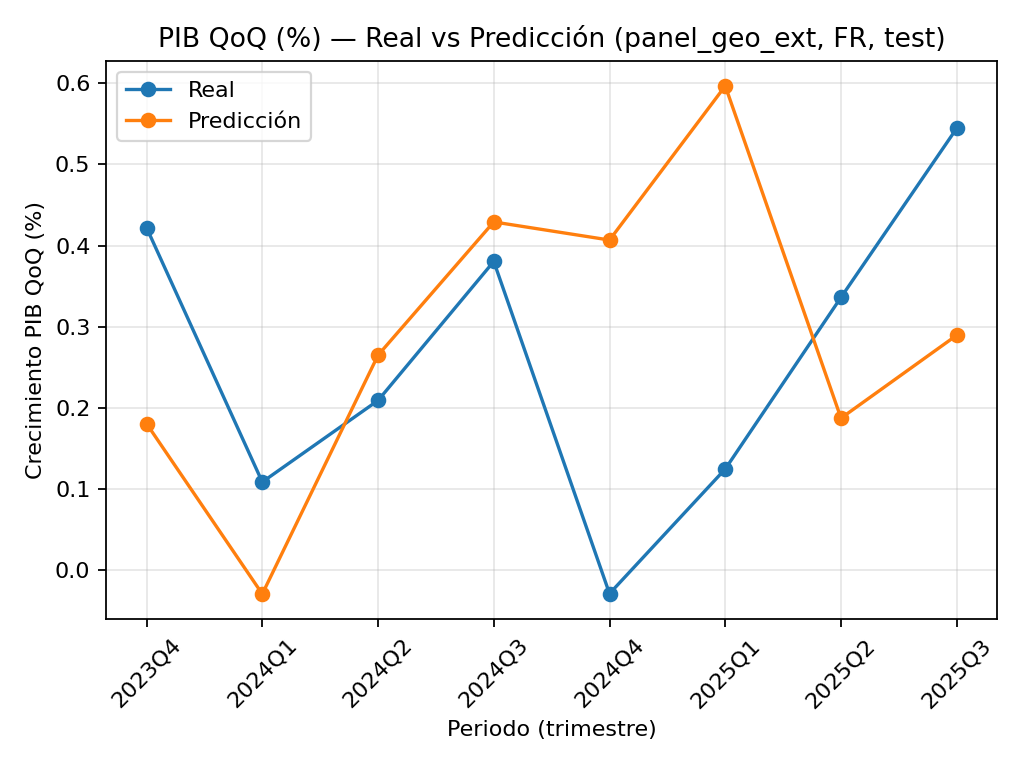
\includegraphics[width=\textwidth]{figures/bloque 2/panel_geo_ext_fr_real_vs_pred.png}
    \caption{PIB QoQ real vs predicción -- panel geo ampliado (FR, test)}
    \label{fig:b2_ext_fr_pred}
\end{minipage}

\vspace{0.5em}

\begin{minipage}[t]{0.48\textwidth}
    \centering
    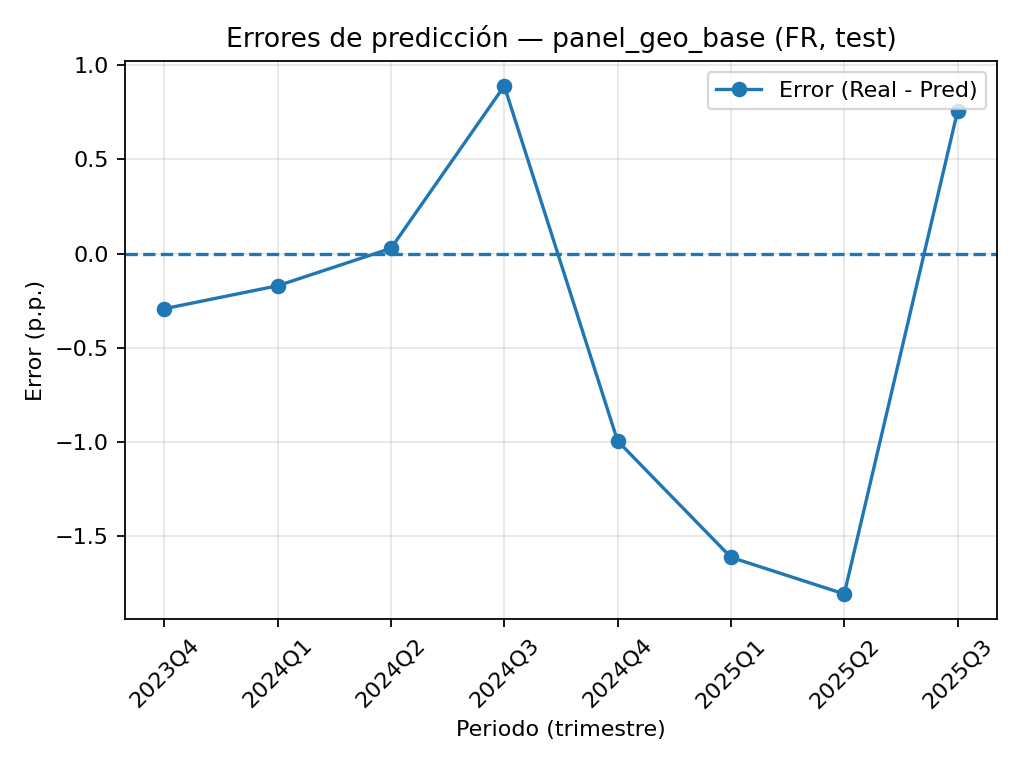
\includegraphics[width=\textwidth]{figures/bloque 2/panel_geo_base_fr_errors.png}
    \caption{Errores de predicción -- panel geo base (FR, test)}
    \label{fig:b2_base_fr_err}
\end{minipage}\hfill
\begin{minipage}[t]{0.48\textwidth}
    \centering
    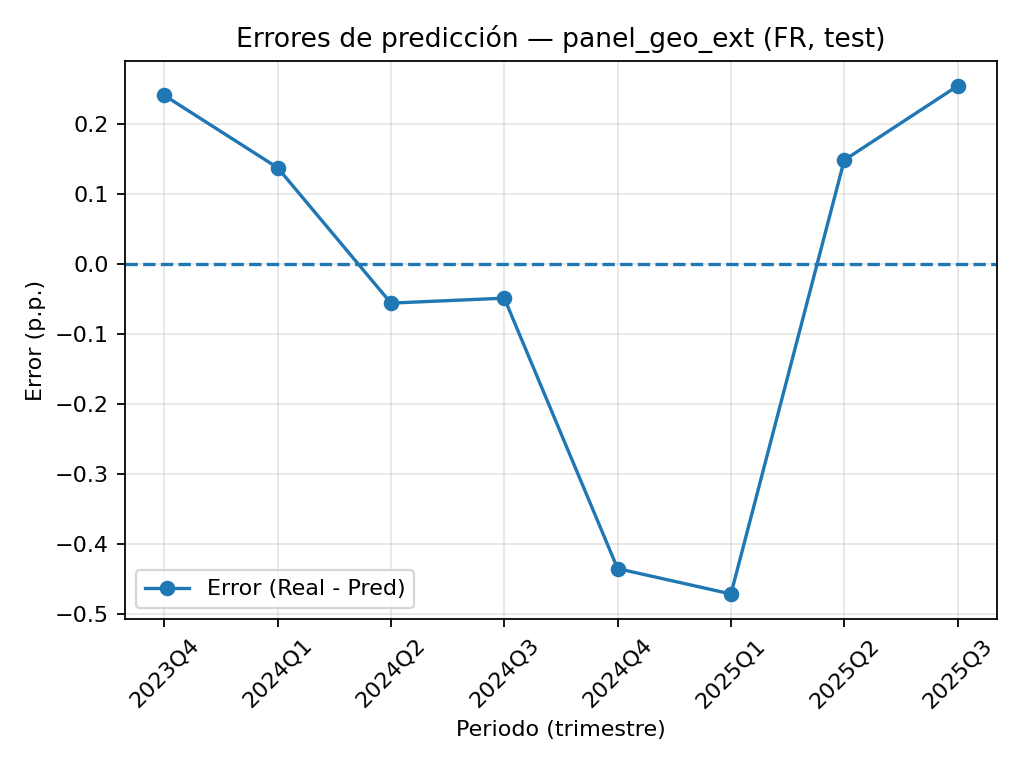
\includegraphics[width=\textwidth]{figures/bloque 2/panel_geo_ext_fr_errors.png}
    \caption{Errores de predicción -- panel geo ampliado (FR, test)}
    \label{fig:b2_ext_fr_err}
\end{minipage}
\end{figure}

\FloatBarrier
\subsection{Italia}

Italia registra el resultado más extremo de todos los experimentos realizados: el modelo base
con dummies de país obtiene un MAE de 4.324 y un RMSE de 6.518, frente a los 0.631 y 1.039
del Bloque~1. La Figura~\ref{fig:b2_base_it_pred} muestra predicciones completamente
desconectadas de la realidad, con valores que alcanzan magnitudes imposibles en el contexto
del crecimiento trimestral. La causa reside en la interacción entre la dummy
\texttt{geo\_IT} y la ausencia de variables autorregresivas: durante el entrenamiento, el
modelo aprende que la combinación de valores bajos de desempleo e inflación rezagados junto
con \texttt{geo\_IT}=1 se corresponde, en algunos trimestres de la recuperación
2020--2022, con crecimientos muy elevados del PIB. Al llegar al periodo de prueba, el modelo
aplica esa regla aprendida fuera del contexto económico que la originó, produciendo
predicciones que ilustran un caso clásico de sobreajuste catastrófico por sobreexplotación
de la señal de identidad categórica.

El modelo ampliado corrige completamente este comportamiento, obteniendo un MAE de 0.365
y un RMSE de 0.451, que supera incluso al modelo ampliado del Bloque~1 (MAE 0.376, RMSE
0.466). La Figura~\ref{fig:b2_ext_it_pred} muestra que el modelo sigue razonablemente la
dirección general del crecimiento italiano, aunque con errores de amplitud en los trimestres
2024Q1 y 2024Q4, donde no anticipa la moderación de la actividad económica. Este patrón,
ya observado en bloques anteriores, apunta a que la dinámica italiana presenta quiebros de
dirección que los retardos del PIB no logran anticipar de forma sistemática.

\begin{figure}[H]
\centering
\begin{minipage}[t]{0.48\textwidth}
    \centering
    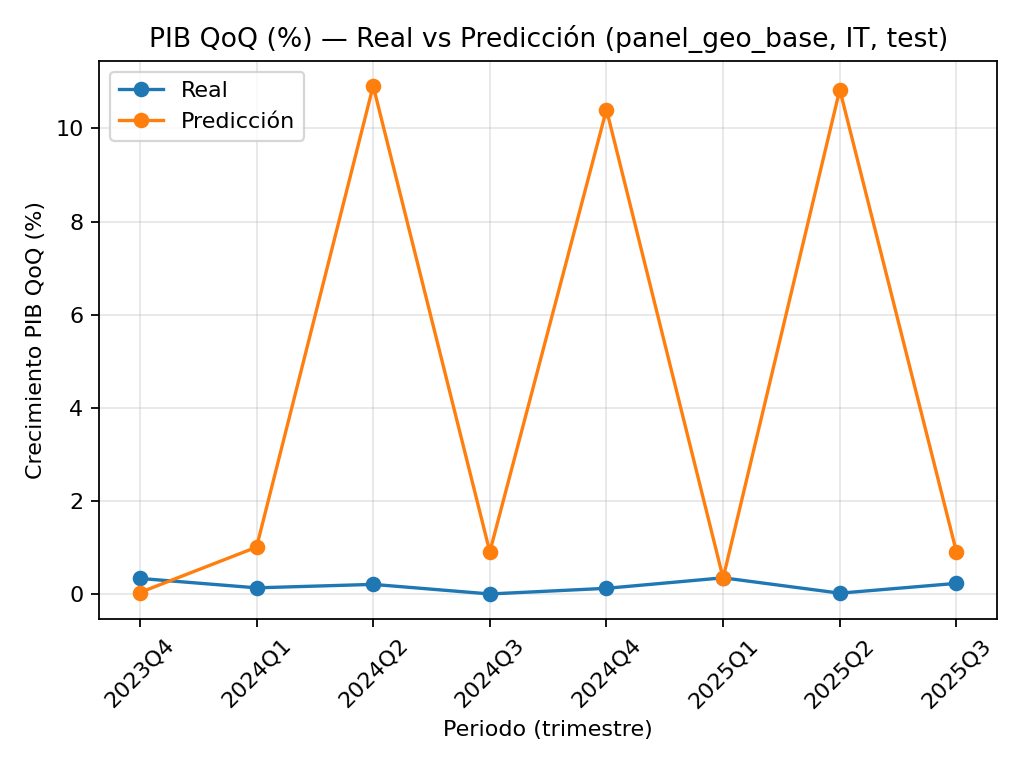
\includegraphics[width=\textwidth]{figures/bloque 2/panel_geo_base_it_real_vs_pred.png}
    \caption{PIB QoQ real vs predicción -- panel geo base (IT, test)}
    \label{fig:b2_base_it_pred}
\end{minipage}\hfill
\begin{minipage}[t]{0.48\textwidth}
    \centering
    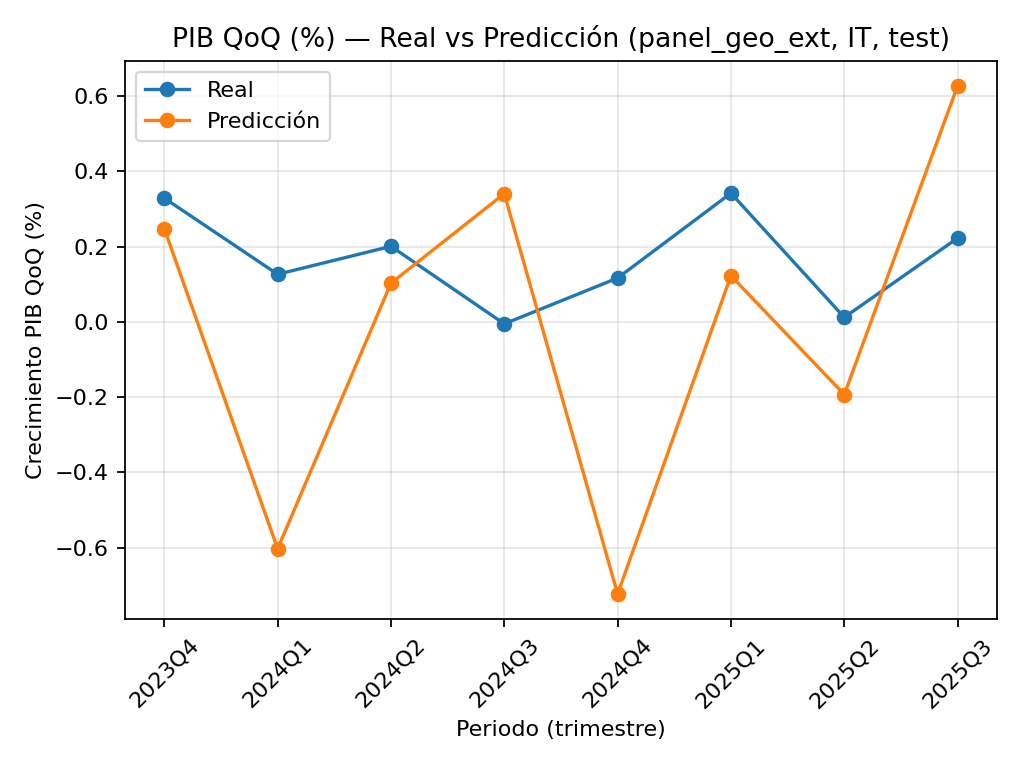
\includegraphics[width=\textwidth]{figures/bloque 2/panel_geo_ext_it_real_vs_pred.png}
    \caption{PIB QoQ real vs predicción -- panel geo ampliado (IT, test)}
    \label{fig:b2_ext_it_pred}
\end{minipage}

\vspace{0.5em}

\begin{minipage}[t]{0.48\textwidth}
    \centering
    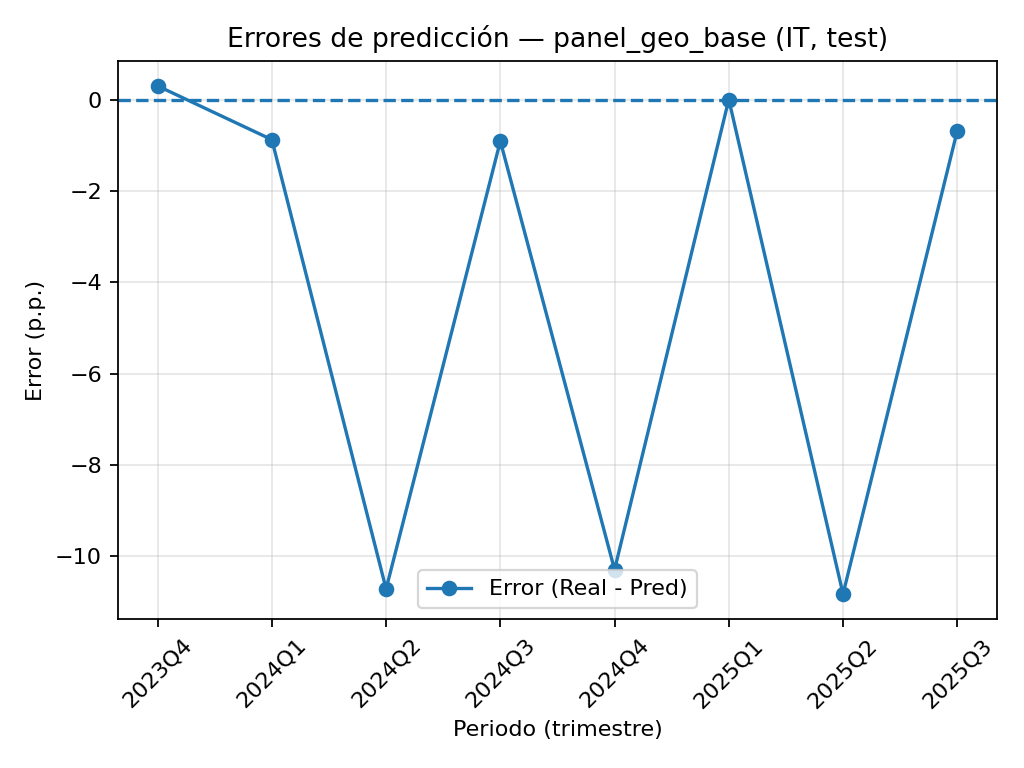
\includegraphics[width=\textwidth]{figures/bloque 2/panel_geo_base_it_errors.png}
    \caption{Errores de predicción -- panel geo base (IT, test)}
    \label{fig:b2_base_it_err}
\end{minipage}\hfill
\begin{minipage}[t]{0.48\textwidth}
    \centering
    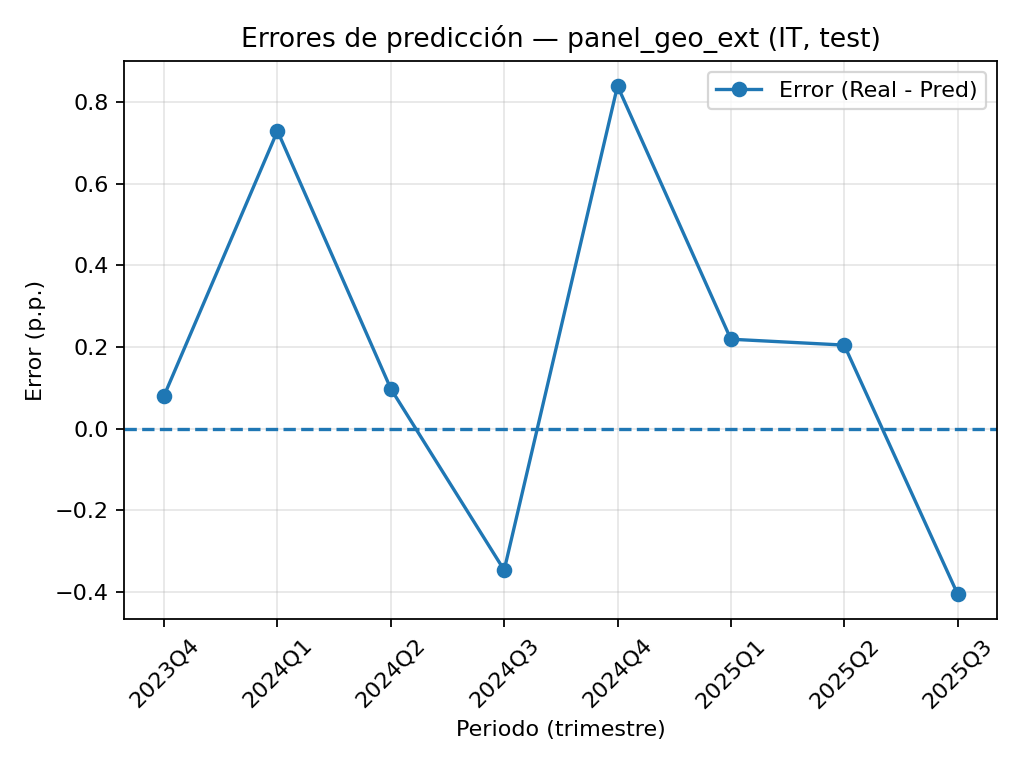
\includegraphics[width=\textwidth]{figures/bloque 2/panel_geo_ext_it_errors.png}
    \caption{Errores de predicción -- panel geo ampliado (IT, test)}
    \label{fig:b2_ext_it_err}
\end{minipage}
\end{figure}

\FloatBarrier
\subsection{Importancia de variables}

Las Figuras~\ref{fig:b2_base_imp} y~\ref{fig:b2_ext_imp} muestran la importancia relativa
de las variables en el modelo panel geo para las configuraciones base y ampliada respectivamente.

En el modelo base (Figura~\ref{fig:b2_base_imp}), las variables económicas
\texttt{unemployment\_\allowbreak{}rate\_\allowbreak{}l1} e \texttt{inflation\_\allowbreak{}qoq\_\allowbreak{}pct\_\allowbreak{}l1} siguen ocupando los
primeros puestos, tal y como ocurría en el Bloque~1. Sin embargo, la novedad más reveladora
es que \texttt{geo\_FR} ocupa el tercer lugar con una ganancia notablemente superior a la de
\texttt{geo\_ES} y \texttt{geo\_IT}. Esta jerarquía explica directamente el deterioro de
las predicciones francesas: el modelo dedica una fracción significativa de su capacidad de
división a identificar si la observación pertenece a Francia, asociando esa identidad a un
nivel de crecimiento elevado que no se corresponde con el periodo de prueba.

En el modelo ampliado (Figura~\ref{fig:b2_ext_imp}), el retardo inmediato del PIB
(\texttt{gdp\_\allowbreak{}qoq\_\allowbreak{}pct\_\allowbreak{}l1}) concentra de nuevo la mayor parte de la importancia
explicativa, reproduciendo el patrón dominante ya observado en los Bloques~0 y~1. El
resultado más importante desde la perspectiva de este bloque es que las tres dummies de
país presentan ganancias marginales, inferiores a 0.3 frente a las $\approx$16 unidades del
retardo del PIB. Una vez disponibles los retardos del PIB y los indicadores de actividad,
el modelo prácticamente ignora la información de identidad nacional, lo que sugiere que la
información geográfica podría estar ya codificada de forma implícita en la dinámica autorregresiva
de cada economía.

\begin{figure}[H]
\centering
\begin{minipage}[t]{0.48\textwidth}
    \centering
    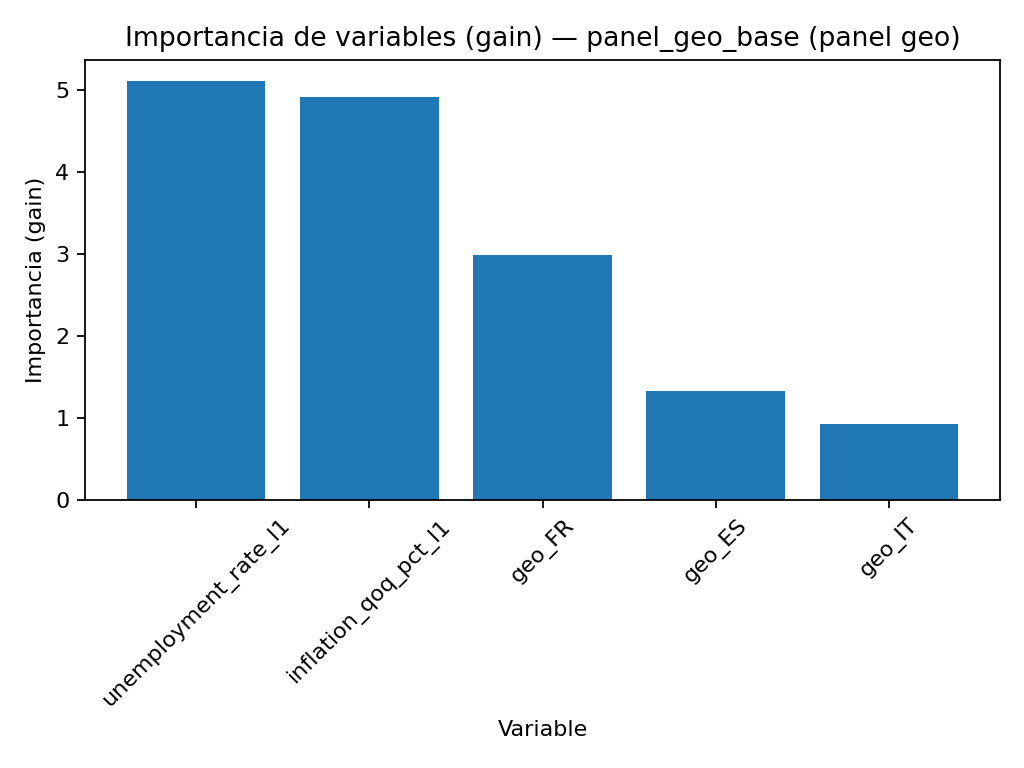
\includegraphics[width=\textwidth]{figures/bloque 2/panel_geo_base_combined_feature_importance.png}
    \caption{Importancia de variables (gain) -- panel geo base}
    \label{fig:b2_base_imp}
\end{minipage}\hfill
\begin{minipage}[t]{0.48\textwidth}
    \centering
    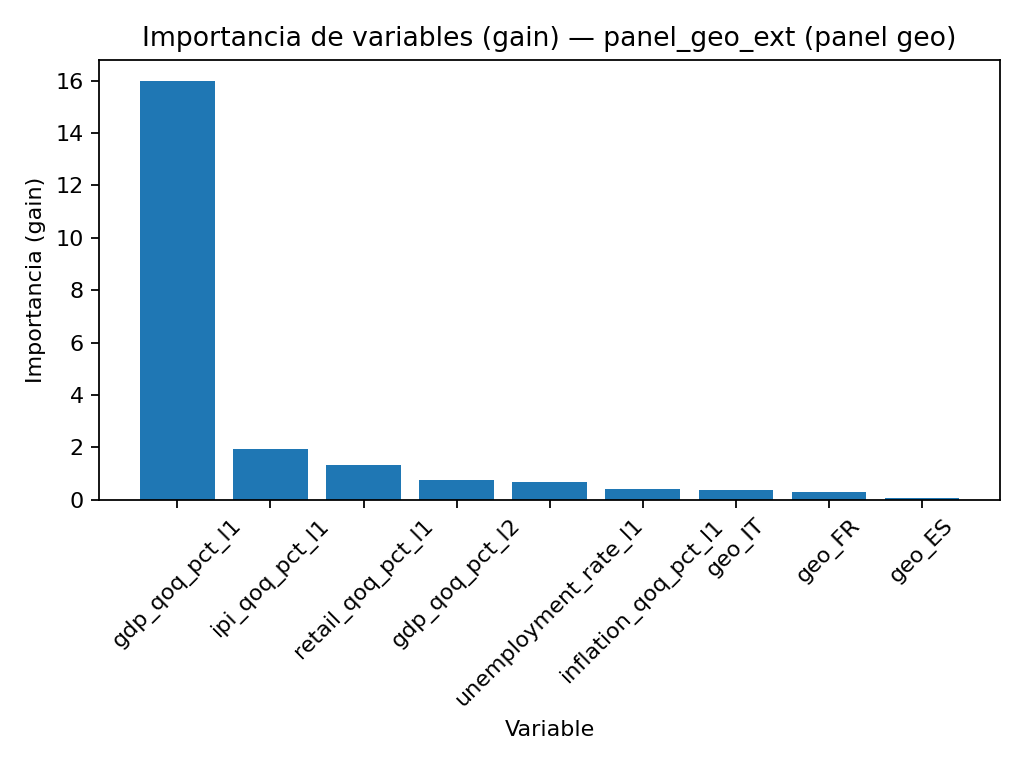
\includegraphics[width=\textwidth]{figures/bloque 2/panel_geo_ext_combined_feature_importance.png}
    \caption{Importancia de variables (gain) -- panel geo ampliado}
    \label{fig:b2_ext_imp}
\end{minipage}
\end{figure}

\FloatBarrier
\subsection{Síntesis del Bloque 2}

Los resultados del Bloque~2 revelan que la codificación de la variable de país como feature
es un arma de doble filo cuya eficacia depende críticamente de las variables económicas
disponibles en el modelo.

Cuando el modelo cuenta con los retardos del PIB y los indicadores de actividad
---configuración ampliada---, las dummies de país no aportan capacidad predictiva adicional
apreciable pero tampoco perjudican: los resultados son prácticamente idénticos a los del
Bloque~1 o ligeramente superiores en España e Italia. En este escenario, la identidad
geográfica queda subsumida por la información autorregresiva, que ya codifica de forma
implícita las diferencias de nivel y volatilidad entre economías.

En cambio, cuando el modelo base carece de esa información de anclaje, las dummies de
país se convierten en la señal más distintiva disponible y el modelo las sobreexplota. El
resultado es una regresión hacia medias de entrenamiento específicas de cada país que ya no
son representativas del periodo de prueba, con un deterioro especialmente grave en Francia
y un colapso catastrófico en Italia (MAE 4.324 frente a 0.631 en el Bloque~1).

Desde una perspectiva metodológica, este experimento apunta a que las variables de
identidad categórica ---país, sector, empresa--- en modelos de series temporales
macroeconómicas podrían ser secundarias respecto a las variables de estado autorregresivas. El nivel
reciente de actividad económica es un predictor mucho más informativo que la etiqueta del
país al que pertenece la observación, y ningún mecanismo de codificación categórica puede
sustituir esa información cuando no está disponible.

El modelo ampliado del Bloque~2 (\texttt{panel\_geo\_ext}) obtiene el mejor MAE para
España (0.290) y para Italia (0.365) de todos los bloques hasta este punto, y un resultado
prácticamente idéntico al Bloque~1 en Francia (0.224 frente a 0.215). Estos resultados
motivan la exploración del Bloque~3, donde se analiza la capacidad de transferencia entre
economías entrenando con los datos de dos países y evaluando sobre el tercero.

% ══════════════════════════════════════════════════════════════════════
\FloatBarrier
\section{Bloque 3 --- Transferencia entre países}

\textbf{Idea principal:} entrenar con dos países y evaluar en un tercero que no ha
participado en el entrenamiento produce resultados sorprendentemente competitivos,
sugiriendo que los patrones macroeconómicos del ciclo trimestral son parcialmente
transferibles entre las economías analizadas.

En los bloques anteriores el país de evaluación siempre había aportado datos al
entrenamiento. El Bloque~3 rompe esta condición: se entrena un modelo XGBoost con la
configuración ampliada usando los datos de dos países y se evalúa sobre el tercero, que
no ha sido visto en ninguna fase del ajuste del modelo. Este diseño permite explorar si
los patrones macroeconómicos aprendidos de dos economías son lo suficientemente generales
como para generalizar a una tercera.

Se ejecutan las tres combinaciones posibles:

\begin{itemize}
    \item \textbf{ES + FR → IT}: entrena con España y Francia, evalúa en Italia.
    \item \textbf{ES + IT → FR}: entrena con España e Italia, evalúa en Francia.
    \item \textbf{FR + IT → ES}: entrena con Francia e Italia, evalúa en España.
\end{itemize}

En todos los casos se utiliza la configuración de features ampliada
(\texttt{gdp\_qoq\_pct\_l1}, \texttt{gdp\_qoq\_pct\_l2}, \texttt{unemployment\_rate\_l1},
\texttt{inflation\_qoq\_pct\_l1}, \texttt{ipi\_qoq\_pct\_l1}, \texttt{retail\_qoq\_pct\_l1}),
la misma partición temporal y los mismos hiperparámetros XGBoost de los bloques anteriores.
La configuración base no se incluye en este bloque dado que su rendimiento sin variables
autorregresivas fue consistentemente inferior en todos los experimentos previos.

Los resultados obtenidos son los siguientes:

\begin{table}[H]
\centering
\caption{Resultados del Bloque 3 --- Transferencia entre países (modelo ampliado)}
\label{tab:bloque3}
\small
\begin{tabular}{llcc}
\hline
\textbf{Entrenado con} & \textbf{Evaluado en} & \textbf{MAE} & \textbf{RMSE} \\
\hline
ES + FR & Italia  & 0.311 & 0.344 \\
ES + IT & Francia & 0.220 & 0.362 \\
FR + IT & España  & 0.337 & 0.367 \\
\hline
\end{tabular}
\end{table}

Para contextualizar estos valores, la Tabla~\ref{tab:comparativa_final} recoge los
resultados del modelo ampliado en todos los bloques para los tres países.

\begin{table}[H]
\centering
\caption{Comparativa del modelo ampliado entre todos los bloques}
\label{tab:comparativa_final}
\small
\begin{tabular}{lcccccc}
\hline
 & \multicolumn{2}{c}{\textbf{España}} & \multicolumn{2}{c}{\textbf{Francia}} & \multicolumn{2}{c}{\textbf{Italia}} \\
\textbf{Bloque} & \textbf{MAE} & \textbf{RMSE} & \textbf{MAE} & \textbf{RMSE} & \textbf{MAE} & \textbf{RMSE} \\
\hline
B0 — Por país       & 0.796 & 1.285 & 0.193 & 0.208 & 0.344 & 0.455 \\
B1 — Panel combinado & 0.297 & 0.331 & 0.215 & 0.256 & 0.376 & 0.466 \\
B2 — Panel con geo  & 0.290 & 0.331 & 0.224 & 0.270 & 0.365 & 0.451 \\
B3 — Transferencia  & 0.337 & 0.367 & 0.220 & 0.362 & 0.311 & 0.344 \\
\hline
\end{tabular}
\end{table}

\FloatBarrier
\subsection{Italia (ES+FR → IT)}

Italia es el resultado más llamativo del bloque. El modelo entrenado exclusivamente con
datos de España y Francia obtiene un MAE de 0.311 sobre Italia, mejorando tanto el
resultado del Bloque~0 con datos italianos propios (MAE 0.344) como los de los Bloques~1
y~2 (0.376 y 0.365 respectivamente). Este resultado apunta a que los patrones del ciclo
económico trimestral de España y Francia capturan regularidades compartidas con Italia
que no quedaban bien representadas cuando el modelo disponía únicamente de las~58
observaciones italianas de entrenamiento.

La Figura~\ref{fig:b3_it_pred} muestra que el modelo sigue razonablemente la dirección
del crecimiento italiano, sin producir predicciones anómalas extremas como las observadas
en el modelo base del Bloque~2.

\begin{figure}[H]
\centering
\begin{minipage}[t]{0.48\textwidth}
    \centering
    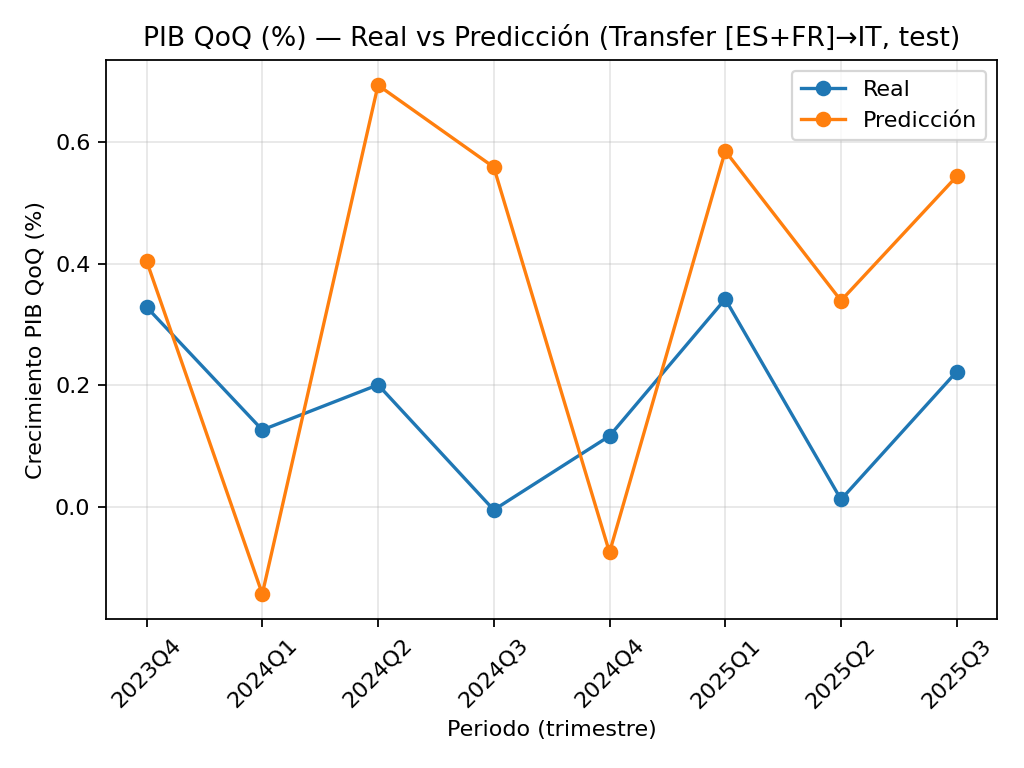
\includegraphics[width=\textwidth]{figures/bloque 3/panel_transfer_ext_it_real_vs_pred.png}
    \caption{PIB QoQ real vs predicción -- Transfer ES+FR → IT (test)}
    \label{fig:b3_it_pred}
\end{minipage}\hfill
\begin{minipage}[t]{0.48\textwidth}
    \centering
    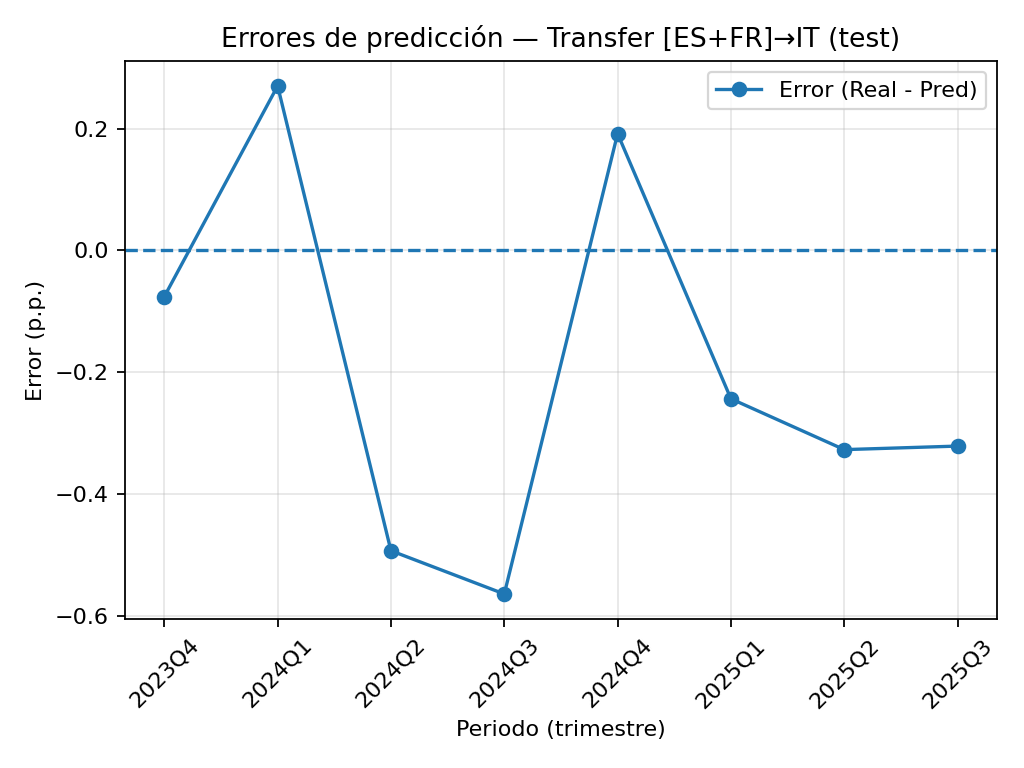
\includegraphics[width=\textwidth]{figures/bloque 3/panel_transfer_ext_it_errors.png}
    \caption{Errores de predicción -- Transfer ES+FR → IT (test)}
    \label{fig:b3_it_err}
\end{minipage}
\end{figure}

\FloatBarrier
\subsection{Francia (ES+IT → FR)}

Francia obtiene un MAE de 0.220 en transferencia, prácticamente idéntico al 0.215 del
Bloque~1. Este resultado sugiere que los patrones de España e Italia son suficientes para
estimar el crecimiento francés con una precisión comparable a la del modelo entrenado con
todos los países, incluyendo Francia. La Figura~\ref{fig:b3_fr_pred} muestra un ajuste
similar al de bloques anteriores, con errores contenidos en la mayor parte del horizonte
de prueba.

\begin{figure}[H]
\centering
\begin{minipage}[t]{0.48\textwidth}
    \centering
    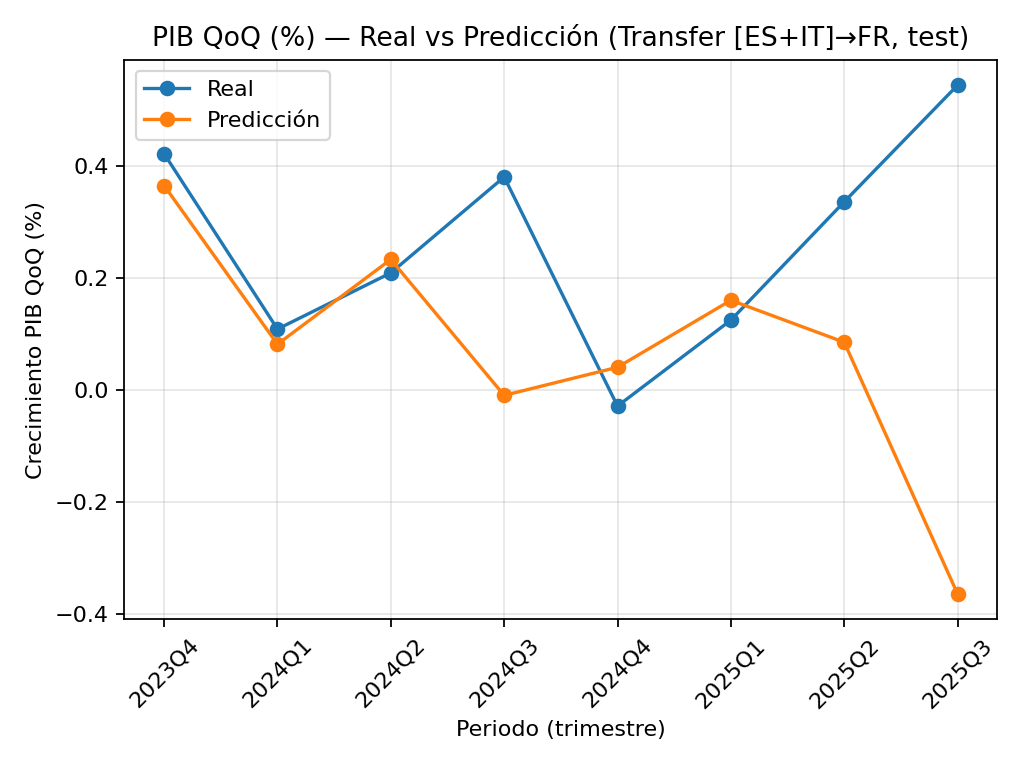
\includegraphics[width=\textwidth]{figures/bloque 3/panel_transfer_ext_fr_real_vs_pred.png}
    \caption{PIB QoQ real vs predicción -- Transfer ES+IT → FR (test)}
    \label{fig:b3_fr_pred}
\end{minipage}\hfill
\begin{minipage}[t]{0.48\textwidth}
    \centering
    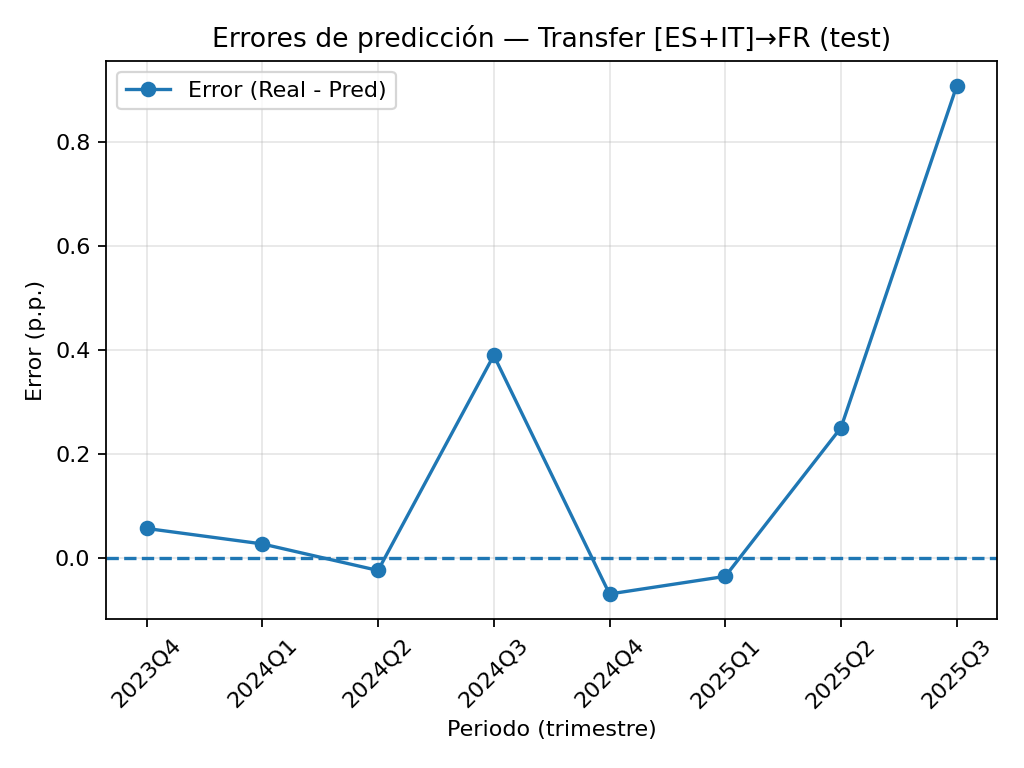
\includegraphics[width=\textwidth]{figures/bloque 3/panel_transfer_ext_fr_errors.png}
    \caption{Errores de predicción -- Transfer ES+IT → FR (test)}
    \label{fig:b3_fr_err}
\end{minipage}
\end{figure}

\FloatBarrier
\subsection{España (FR+IT → ES)}

España obtiene un MAE de 0.337 en transferencia, superior al 0.290--0.297 de los
Bloques~1 y~2, pero muy por debajo del 0.796 que obtenía el modelo ampliado del Bloque~0
con datos españoles propios. La Figura~\ref{fig:b3_es_pred} muestra que el modelo captura
la tendencia general del crecimiento español, aunque con mayor imprecisión que cuando
disponía de datos nacionales en el entrenamiento.

\begin{figure}[H]
\centering
\begin{minipage}[t]{0.48\textwidth}
    \centering
    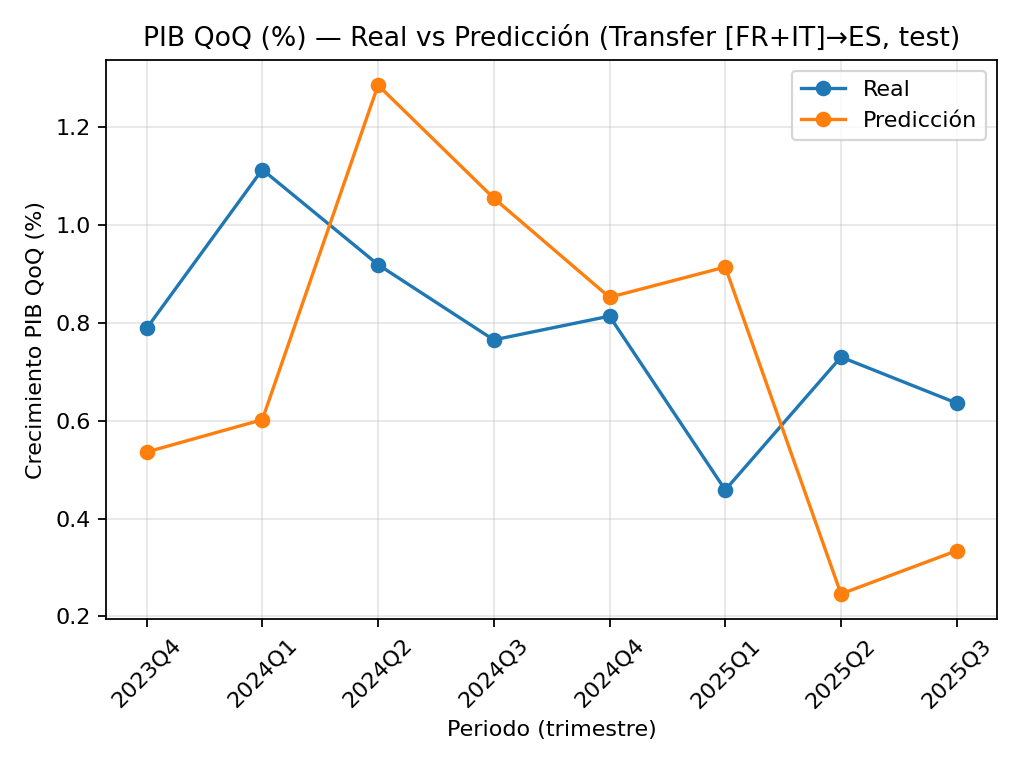
\includegraphics[width=\textwidth]{figures/bloque 3/panel_transfer_ext_es_real_vs_pred.png}
    \caption{PIB QoQ real vs predicción -- Transfer FR+IT → ES (test)}
    \label{fig:b3_es_pred}
\end{minipage}\hfill
\begin{minipage}[t]{0.48\textwidth}
    \centering
    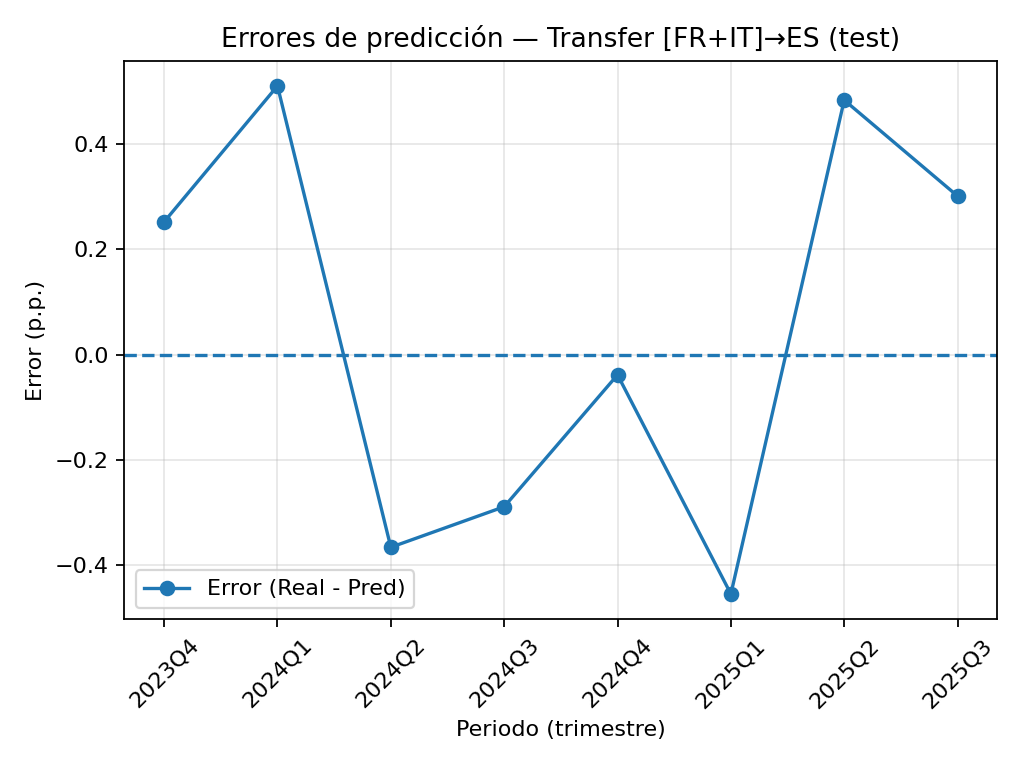
\includegraphics[width=\textwidth]{figures/bloque 3/panel_transfer_ext_es_errors.png}
    \caption{Errores de predicción -- Transfer FR+IT → ES (test)}
    \label{fig:b3_es_err}
\end{minipage}
\end{figure}

\FloatBarrier
\subsection{Síntesis del Bloque 3}

Los resultados del Bloque~3 apuntan a que los patrones macroeconómicos del ciclo
trimestral presentan un grado de transferibilidad entre estas tres economías europeas
mayor del que cabría esperar a priori. En los tres experimentos el modelo obtiene errores
competitivos sin haber visto ningún dato del país de evaluación durante el entrenamiento.

El hallazgo más destacado es el de Italia: el modelo entrenado con ES+FR parece generalizar
mejor a Italia que los modelos entrenados con datos italianos propios en los Bloques~0,
1 y~2. Esto sugiere que la limitada cantidad de observaciones italianas disponibles
introduce más ruido que señal en los bloques donde Italia participa en el entrenamiento,
y que los patrones de España y Francia capturan regularidades cíclicas compartidas que
resultan útiles para estimar el crecimiento italiano.

Para Francia y España, la transferencia produce resultados ligeramente inferiores a los
de los bloques con datos propios (Bloques~1 y~2), lo que es coherente con lo esperado:
la información del propio país durante el entrenamiento aporta valor, pero su ausencia
no impide que el modelo mantenga una capacidad predictiva razonable.

En conjunto, estos resultados apuntan a que los lags del PIB y los indicadores de
actividad económica codifican regularidades del ciclo macroeconómico que son
parcialmente compartidas entre estas economías, lo que podría tener implicaciones
prácticas en contextos donde los datos históricos de un país son escasos o de baja
calidad.